\chapter{Areal quantities in the cortex}
\label{sec:areal}
\setstretch{\lspac}

\section{Introduction}

The surface area of the cerebral cortex greatly differs across species, whereas the cortical thickness has remained relatively constant during evolution \citep{Mountcastle1998, Fish2008}. At a microanatomic scale, regional morphology is closely related to functional specialization \citep{Roland1998, Zilles2010}, contrasting with the columnar organization of the cortex, in which cells from different layers respond to the same stimulus \citep{EGJones2000, Buxhoeveden2002}. In addition, \citet{Rakic1988} proposed an ontogenetic model that explains the processes that lead to cortical arealization and differentiation of cortical layers according to related, yet independent mechanisms. Supporting evidence for this model has been found in studies with both rodent and primates, including humans \citep{Chenn2002, Rakic2009}, as well as in pathological states \citep{Rimol2010b, Bilguvar2010}.

At least some of the variability of the distinct genetic and developmental processes that seem to determine regional cortical area and thickness can be captured using polygon mesh (surface-based) representations of the cortex derived from $T_1$-weighted magnetic resonance imaging (\textsc{mri}) \citep{Panizzon2009, Winkler2010, SanabriaDiaz2010}. In contrast, volumetric (voxel-based) representations, also derived from \textsc{mri}, were shown to be unable to readily disentangle these processes \citep{Winkler2010}. Figure~\ref{fig:areal:geometry} shows schematically the difference between these two representations.

\begin{figure}[!tp]
\centering
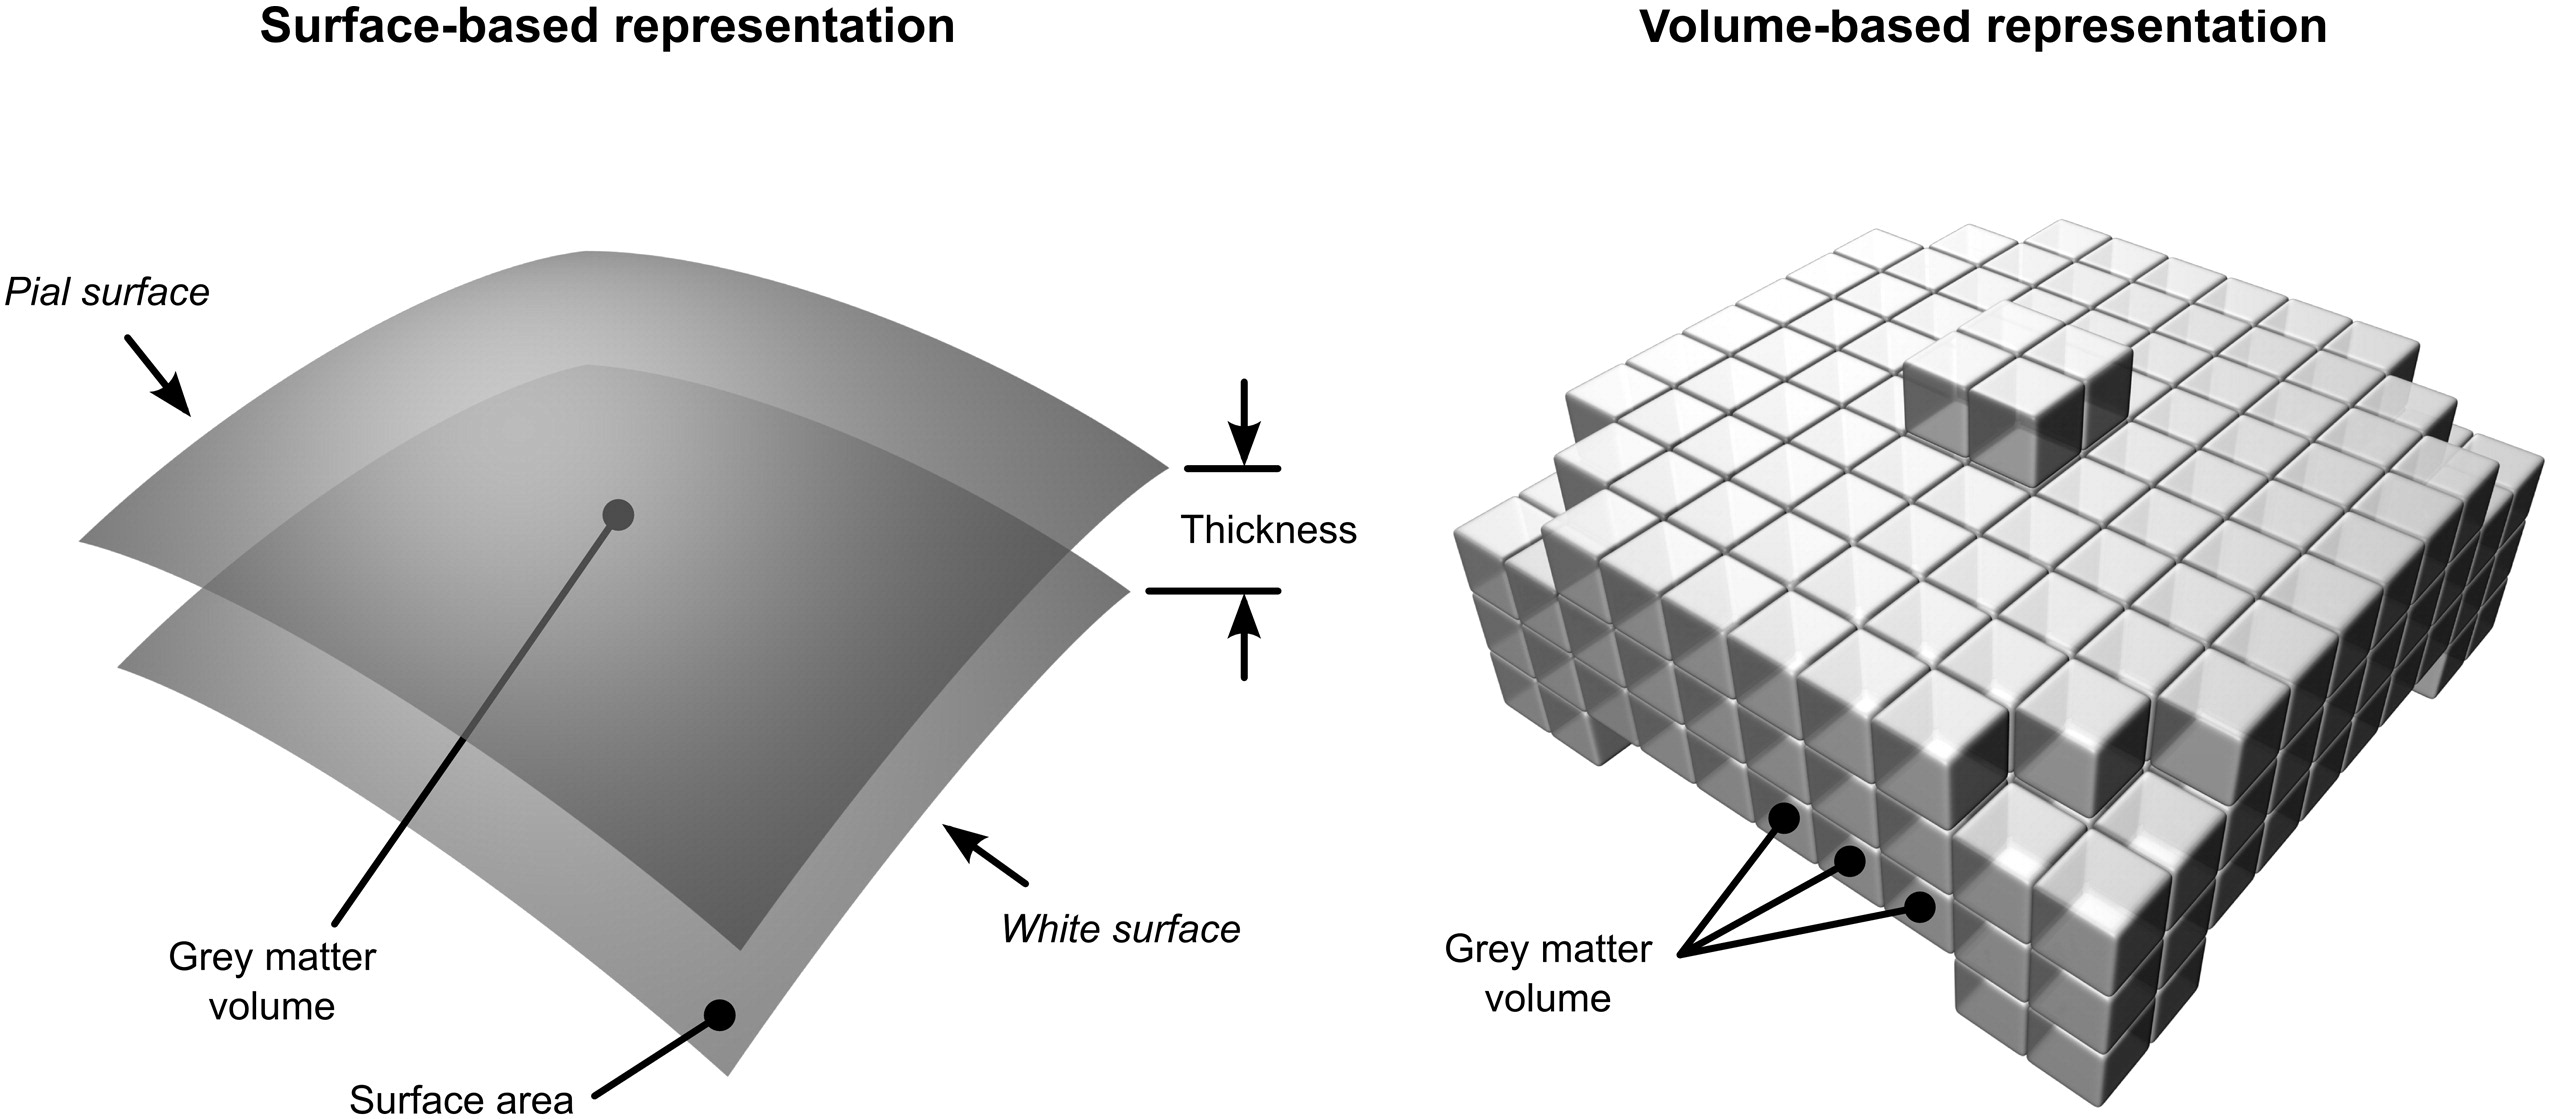
\includegraphics[width=14cm]{images/geometry.jpg}
\caption[Surface- and volume-based representations of the cortex.]{Geometrical relationship between cortical thickness, surface area and grey matter volume. In the surface-based representation, the grey matter volume is a quadratic function of distances in the surfaces and a linear function of the thickness. In the volume-based representation, only the volumes can be measured directly and require partial volume-effects to be considered \citep{Winkler2010}.}
\label{fig:areal:geometry}
\end{figure}

Mesh representations of the brain allow measurements of the cortical thickness at every point in the cortex, as well as estimation of the average thickness for pre-specified regions. However, to date, analyses of cortical surface area have been generally limited to two types of studies: (1) vertexwise comparisons with a standard brain, using some kind of expansion or contraction measurement, either of the surface itself \citep{Joyner2009, Lyttelton2009, Hill2010, Rimol2010b, Palaniyappan2011}, of linear distances between points in the brain \citep{Sun2009a, Sun2009}, or of geometric distortion \citep{Wisco2007}, or (2) analyses of the area of regions of interest (\textsc{roi}) defined from postulated hypotheses or from macroscopic morphological landmarks \citep{Dickerson2009, Nopoulos2010, Kahler2011, Durazzo2011, Schwarzkopf2011, Eyler2011, Chen2011_neuron, Chen2012}. Analyses of expansion, however, do not deal with area directly, depending instead on non-linear functions associated with the warp to match the standard brain, such as the Jacobian of the transformation. Moreover, by not quantifying the amount of area, these analyses are only interpretable with respect to the brain used for the comparisons. R\textsc{oi}-based analyses, on the other hand, entail the assumption that each region is homogeneous with regard to the feature under study, and have maximum sensitivity only when the effect of interest is present throughout the \textsc{roi}.

These difficulties can be obviated by analysing each point on the cortical surface of the mesh representation, a method already well established for cortical thickness \citep{Fischl2000}. Pointwise measurements, such as thickness, are generally taken at and assigned to each vertex of the mesh representation of the cortex. This kind of measurement can be transferred to a common grid and subjected to statistical analysis. Standard interpolation techniques, such as nearest neighbor, barycentric \citep{Yiu2000}, spline-based \citep{DeBoor1962} or distance-weighted \citep{Shepard1968} can be used for this purpose. The resampled data can be further spatially smoothed to alleviate residual interpolation errors. However, this approach is not suitable for areal measurements, since area is not inherently a point feature. To illustrate this aspect, an example is given in Figure~\ref{fig:areal:forest}. Methods that can be used for interpolation of point features do not necessarily compensate for inclusion or removal of datapoints,\footnote{A notable exception is the natural neighbor method \citep{Sibson1981}. However, the original method needs modification for use with areal analyses.} unduly increasing or reducing the global or regional sum of the quantities under study, precluding them for use with measurements that are, by nature, areal. The main contribution of this chapter is to address the technical difficulties in analysing the local brain surface area, \emph{as well as any other cortical quantity that is areal by nature}. We propose a framework to analyse areal quantities and argue that a mass preserving interpolation method is a necessary step. We also study different processing strategies and characterize the distribution of \emph{facewise} cortical surface area.

\begin{figure}[!p]  % Figure 1
\centering
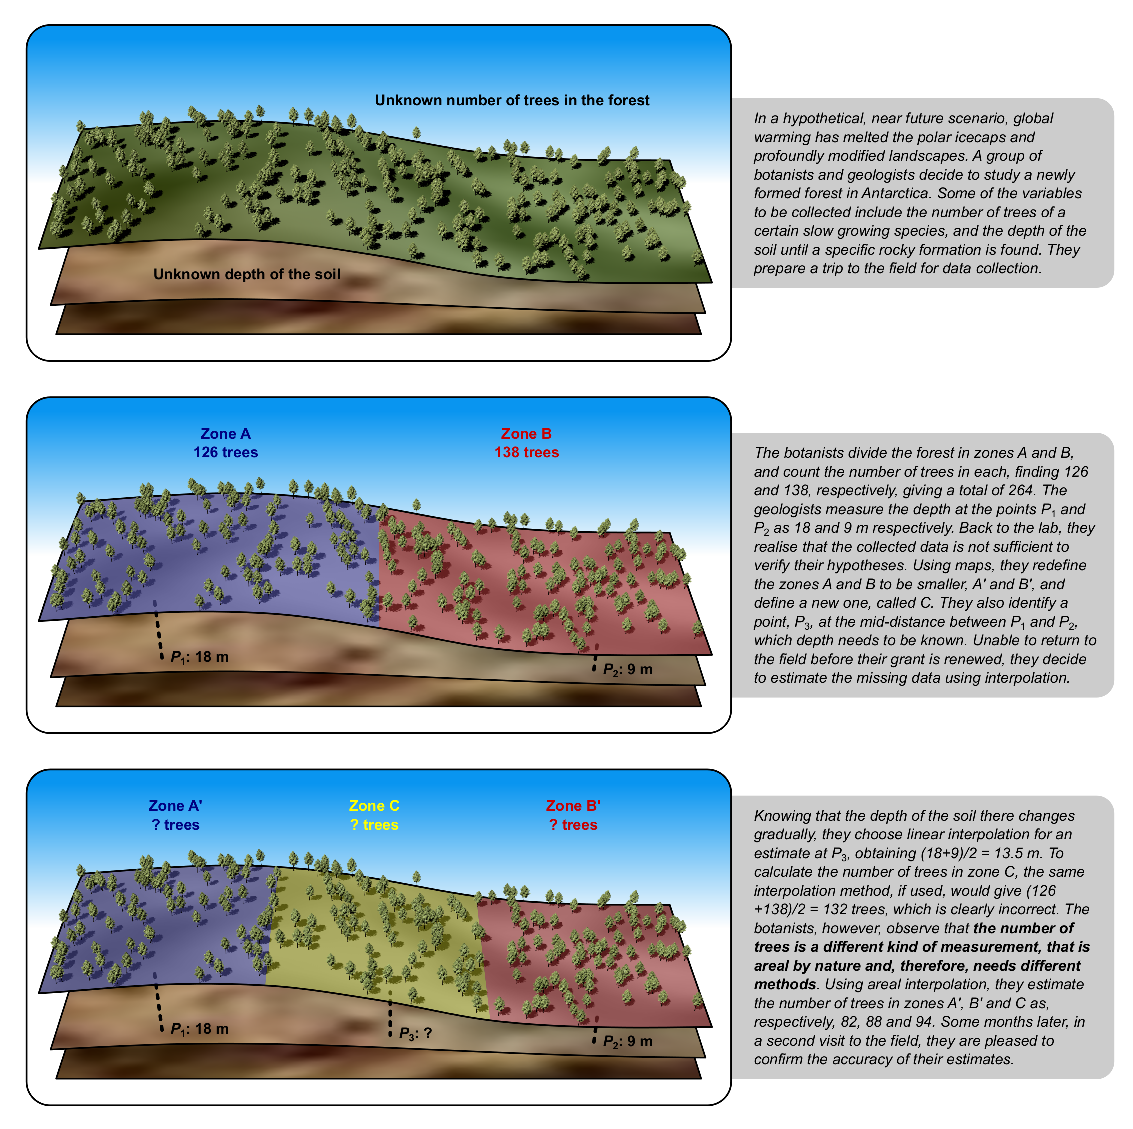
\includegraphics[width=14cm]{images/forest.eps}
\caption[Example demonstrating differences between area and point measurements.]{An example demonstrating differences in the nature of measurements. In this analogy, the depth of the soil is similar to brain cortical thickness, whereas the number of trees is similar to areal quantities distributed across the cortex. These areal quantities can be the surface area itself (in this case, the area of the terrain), but can also be any other measurement that is areal by nature (such as the number of trees).}
\label{fig:areal:forest}
\end{figure}

\section{Method}

An overview of the method is presented in Figure~\ref{fig:areal:overview}. Comparisons of cortical area between subjects require a surface model for the cortex to be constructed. A number of approaches are available \citep{Mangin1995, Dale1999, vanEssen2001, Kim2005} and, in principle, any could be used. Here we adopt the method of \citet{Dale1999} and \citet{Fischl1999_cortical}, as implemented in the FreeSurfer software package (\textsc{fs}).\footnote{Available at \href{http://surfer.nmr.mgh.harvard.edu}{http://surfer.nmr.mgh.harvard.edu}.} In this method, the $T_1$-weighted images are initially corrected for magnetic field inhomogeneities and skull-stripped \citep{Segonne2004}. The voxels belonging to the white matter (\textsc{wm}) are identified based on their locations, on their intensities, and on the intensities of the neighboring voxels. A mass of connected \textsc{wm} voxels is produced for each hemisphere, using a six-neighbors connectivity scheme, and a mesh of triangular faces is tightly built around this mass, using two triangles per exposed voxel face. The mesh is smoothed taking into account the local intensity in the original images \citep{Dale1993}, at a subvoxel resolution. Topological defects are corrected \citep{Fischl2001,Segonne2007} ensuring that the surface has the same topological properties of a sphere. A second iteration of smoothing is applied, resulting in a realistic representation of the interface between gray and white matter (the \emph{white surface}). The external cortical surface (the \emph{pial surface}), which corresponds to the pia mater, is produced by nudging outwards the white surface towards a point where the tissue contrast is maximal, maintaining constraints on its smoothness and on the possibility of self-intersection \citep{Fischl2000}. The white surface is inflated in an area-preserving transformation and subsequently homeomorphically transformed to a sphere \citep{Fischl1999_intersubject}. After the spherical transformation, there is a one-to-one mapping between faces and vertices of the surfaces in the native geometry (white and pial) and the sphere. These surfaces are comprised exclusively of triangular faces.

\begin{figure}[!p]  % Figure 2
\centering
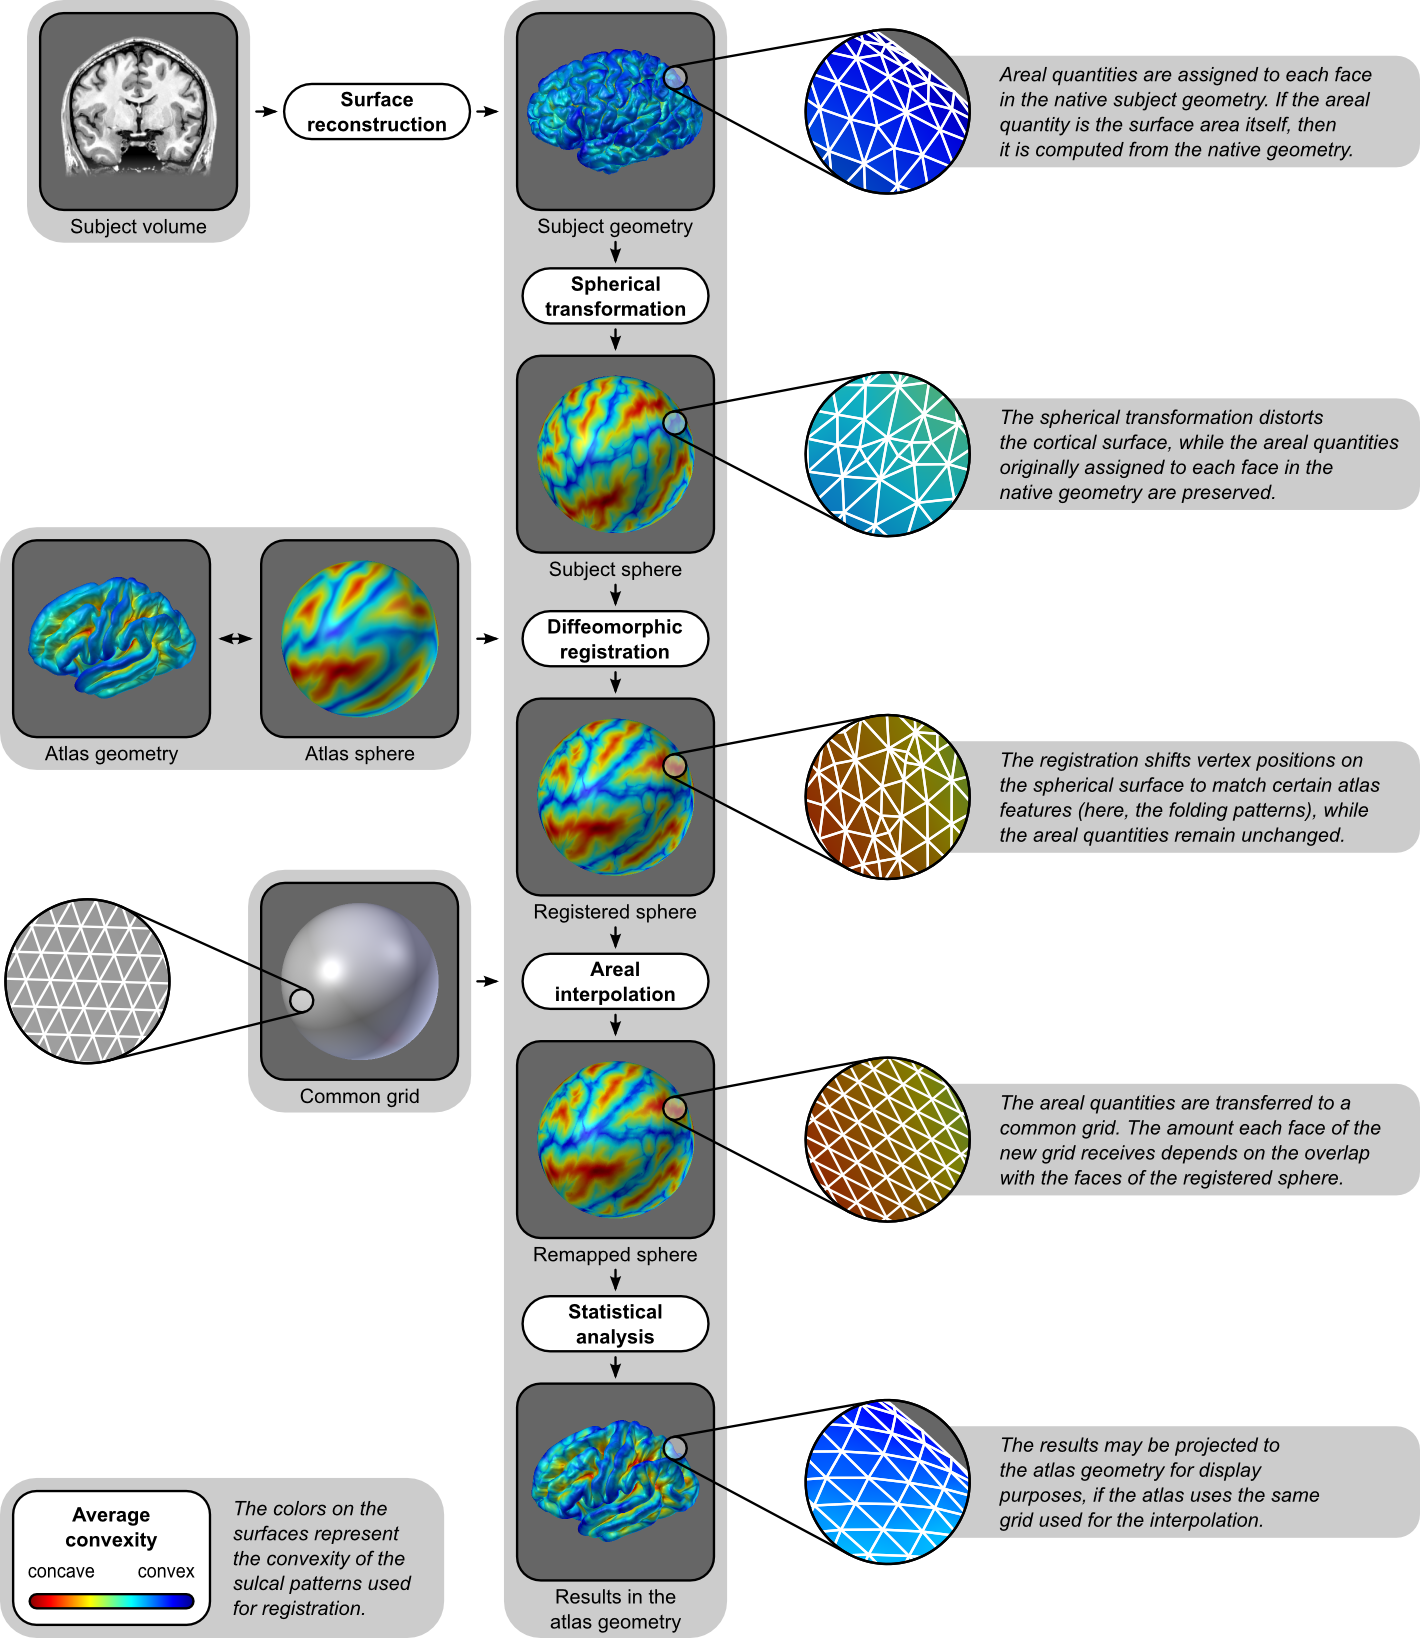
\includegraphics[width=14cm]{images/overview.png}
\caption[Overview of areal analyses.]{Diagram of the steps to analyse the cortical surface area. For clarity, the colors represent the convexity of the surface, as measured in the native geometry.}
\label{fig:areal:overview}
\end{figure}

\subsection{Area per face and other areal quantities}

The surface area for analysis is computed at the interface between gray and white matter, i.e.\ at the \emph{white surface}. Another possible choice is to use the middle surface, i.e.\ a surface that runs at the mid-distance between white and pial. Although this surface is not guaranteed to match any specific cortical layer, it does not over or under-represent gyri or sulci \citep{vanEssen2005}, which might be an useful property. The white surface, on the other hand, matches directly a morphological feature and also tends to be less sensitive to cortical thinning or thickening than the middle or pial surfaces. Whenever methods to produce surfaces that represent biologically meaningful cortical layers are available, these should be preferred.

In contrast to conventional approaches in which the area of all faces that meet at a given vertex is summed and divided by three, producing a measure of the \emph{area per vertex}, for facewise analysis it is the \emph{area per face} that is measured and analysed. Since for each subject, each face in the native geometry has its corresponding face on the sphere, the value that represents area per face, as measured from the native geometry, can be mapped directly to the sphere, despite any areal distortion introduced by the spherical transformation.

Furthermore, since there is a direct mapping that is independent of the actual area in the native geometry, \emph{any other quantity that is biologically areal can also be mapped to the spherical surface}. Perhaps the most prominent example is cortical volume (Section~\ref{sec:areal:volumes}), although other cases of such quantities, that may potentially be better characterized as areal processes, are the extent of the neural activation as observed with functional \textsc{mri}, the amount of amyloid deposited in Alzheimer's disease \citep{Klunk2004, Clark2011}, or simply the the number of cells counted from optic microscopy images reconstructed to a tri-dimensional space \citep{Schormann1998}. Since areal interpolation (described below) conserves locally, regionally and globally the quantities under study, it allows accurate comparisons and analyses across subjects for measurements that are areal by nature, or that require mass conservation on the surface of the mesh representation.

\subsection{Computation of surface area}

The facewise areas in the mesh representation of the brain can be computed trivially: for a triangular face $ABC$ with vertices $\mathbf{a}=[x_A \; y_A \; z_A]'$, $\mathbf{b}=[x_B \; y_B \; z_B]'$, and $\mathbf{c}=[x_C \; y_C \; z_C]'$, the area is $|\mathbf{u} \times \mathbf{v}|/2$, where $\mathbf{u} = \mathbf{a}-\mathbf{c}$, $\mathbf{v} = \mathbf{b}-\mathbf{c}$, $\times$ represents the cross product, and $|\bullet|$ represents the vector norm.

\subsection{Volume as an areal quantity}
\label{sec:areal:volumes}

Gray matter volume can be assessed using the partial volume effects of the gray matter in a per-voxel fashion using volume-based representations of the brain, such as in voxel-based morphometry \citep[\textsc{vbm}][]{Ashburner2000}, or as the amount of tissue present between the gray and white surfaces in surface-based representations. Using the surface-based representation, software such as FreeSurfer up to version 5.3.0 compute the volume through the following steps:

\begin{enumerate}
\item The area at each vertex is computed as $\sfrac{1}{3}$ of the sum of the areas of all faces of the white surface that have that vertex in common. 
\item The volume is computed as the product of the area by the thickness at that vertex.
\end{enumerate}

This procedure, while providing a good approximation that is already superior to volume-based measurements for not being as susceptible to various artefacts that can affect the latter \citep{Ashburner2009}, is still problematic. Simple multiplication of thickness by area leaves considerable amounts of tissue unmeasured at the gyri, while measuring more than once pieces of tissue in the fundi of sulci. Figure~\ref{fig:areal:mantle} shows a simplification to a two-dimensional case of this phenomenon, that affects differentially, and in opposite directions, sulci and gyri.

\begin{figure}[!tp]
\centering
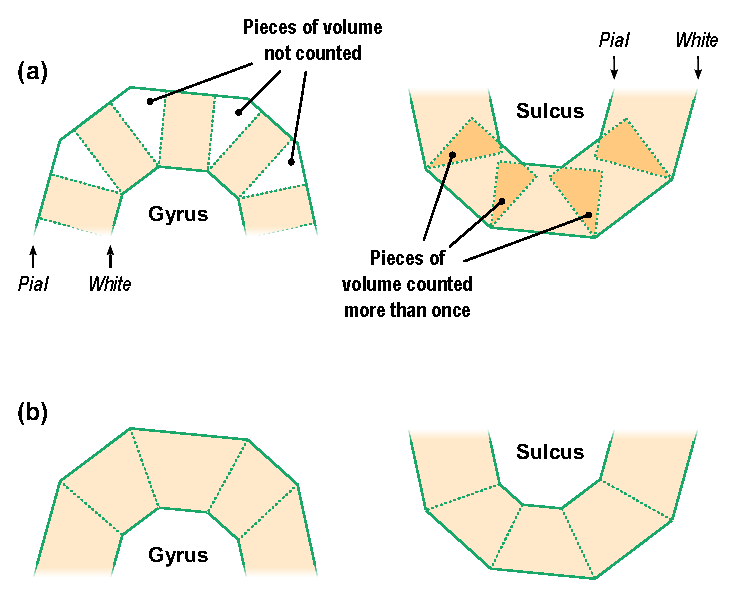
\includegraphics{images/mantle.eps}
\caption[Simple multiplication leaves tissue over- or under-represented.]{(\emph{a}) A simplified two-dimensional representation of the cortex. If the volume is computed using simple multiplication of thickness by area, considerable amount of tissue is left unmeasured in the gyri, or measured more than once in sulci. (\emph{b}) The proposed method, would compute analytically the volumes of the regions of tissue between matching faces of white and pial surfaces, leaving no part of tissue unmeasured.}
\label{fig:areal:mantle}
\end{figure}

The problem can be alleviated to some extent by using the mid-surface as the reference for area, as opposed to the white. Instead, a more exact solution is proposed here. It consists of using the three vertices that define a face in the white surface, and the matching vertices in the pial surface, to define an \emph{oblique truncated triangular pyramid}, which on its turn can be perfectly subdivided into three non-overlapping tetrahedra; the volumes of these are computed analytically, summed and assigned to each face of the surface representation, and used for subsequent analysis. Figure~\ref{fig:areal:pyramid} illustrates the procedure. More specifically, the procedure is as follows:

\begin{figure}[!tp]
\centering
\includegraphics[width=14cm]{images/pyramid.eps}
\caption[Proposed method to compute volumes in the cortex.]{(\emph{a}) In the surface representation, the cortex is limited internally by the white and externally by the pial surface. (\emph{b}) and (\emph{c}) These two surfaces have matching vertices that can be used to delineate an oblique truncated triangular pyramid. (\emph{d}) In the proposed method, the six vertices of this pyramid are used to define three tetrahedra, the volumes of which are computed analytically.}
\label{fig:areal:pyramid}
\end{figure}

\begin{enumerate}
\item For a given face $A_w B_w C_w$ in the white surface, and its corresponding face $A_p B_p C_p$ in the pial surface, define an oblique truncated triangular pyramid using these six vertices.
\item Split this truncated pyramid into three tetrahedra: $T_1 = (A_w,B_w,C_w,A_p)$, $T_2 = (A_p,B_p,C_p,B_w)$, and $T_3 = (A_p,C_p,C_w,B_w)$.
\item For each such tetrahedra, let $\mathbf{a}$, $\mathbf{b}$, $\mathbf{c}$ and $\mathbf{d}$ represent its four vertices in terms of coordinates $[x\;y\;z]'$. Compute the volume as $|\mathbf{u}\cdot(\mathbf{v} \times \mathbf{w})|/6$, where $\mathbf{u} = \mathbf{a}-\mathbf{d}$, $\mathbf{v} = \mathbf{b}-\mathbf{d}$, $\mathbf{w} = \mathbf{c}-\mathbf{d}$, $\times$ represents the cross product, $\cdot$ represents the dot product, and $|\bullet|$ represents the vector norm.
\end{enumerate}

The procedure can be accelerated by setting $\mathbf{d}=A_p$, that is, the common vertex for all three tetrahedra, such that the vector subtractions can happen only once for all three. If vertexwise values are needed, these can be computed as $\sfrac{1}{3}$ of the volumes of all faces that meet at that vertex.

\subsection{Registration}

Registration to a common coordinate system is necessary to allow comparisons across subjects \citep{Drury1996}. The registration is performed by shifting vertex positions along the surface of the sphere until there is a good alignment between subject and template (target) spheres with respect to certain specific features, usually, but not necessarily, the cortical folding patterns. As the vertices move, the areal quantities assigned to the corresponding faces are also moved along the surface. The target for registration should be the less biased as possible in relation to the population under study \citep{Thompson2002}.

A registration method that produces a smooth, i.e.\ spatially differentiable, warp function enables the smooth transfer of areal quantities. A possible way to accomplish this is by using registration methods that are diffeomorphic. A diffeomorphism is an invertible transformation that has the elegant property that it and its inverse are both continuously differentiable \citep{Christensen1996, Miller1997}, minimising the risk of vagaries that would be introduced by the non-differentiability of the warp function.

Diffeomorphic methods are available for spherical meshes \citep{Glaunes2004, Yeo2010, Robinson2014}, and here we adopt the Spherical Demons (\textsc{sd}) algorithm\footnote{Available at \href{http://sites.google.com/site/yeoyeo02/software/sphericaldemonsrelease}{http://sites.google.com/site/yeoyeo02/software/sphericaldemonsrelease}.} \citep{Yeo2010}. \textsc{Sd} extends the Diffeomorphic Demons algorithm \citep{Vercauteren2009} to spherical surfaces. The Diffeomorphic Demons algorithm is a diffeomorphic variant of the efficient, non-parametric Demons registration algorithm \citep{Thirion1998}. \textsc{Sd} exploits spherical vector spline interpolation theory and efficiently approximates the regularization of the Demons objective function via spherical iterative smooting.

Methods that are not diffeomorphic by construction \citep{Fischl1999_intersubject, Auzias2013}, but in practice produce invertible and smooth warps could, in principle, be used for registration for areal analyses. In the Evaluation section we study the performance of different registration strategies as well as the impact of the choice of the template.

\subsection{Areal interpolation}

After the registration, the correspondence between each face on the registered sphere and each face from the native geometry is maintained, and the surface area or other areal quantity under study can be transferred to a common grid, where statistical comparisons between subjects can be performed. The common grid is a mesh which vertices lie on the surface of a sphere. A geodesic sphere, which can be constructed by iterative subdivision of the faces of a regular icosahedron, has many advantages for this purpose, namely, ease of computation, edges of roughly similar sizes and, if the resolution is fine enough, edge lengths that are much smaller than the diameter of the sphere (see Section~\ref{sec:areal:geosphere} for details). These two spheres, i.e.\ the registered, irregular spherical mesh (source), and the common grid (target), typically have different resolutions. The interpolation method must, nevertheless, \emph{conserve the areal quantities}, globally, regionally and locally. In other words, the method has to be \emph{pycnophylactic}\footnote{From Greek \emph{pyknos} = mass, density, and \emph{phylaxis} = guard, protect, preserve, meaning that the method has to be mass conservative.} \citep{Tobler1979}. This is accomplished by assigning, to each face in the target sphere, the areal quantity of all overlapping faces from the source sphere, weighted by the fraction of overlap between them (Figure~\ref{fig:areal:triangles}).

\begin{figure}[!t]  % Figure 3
\centering
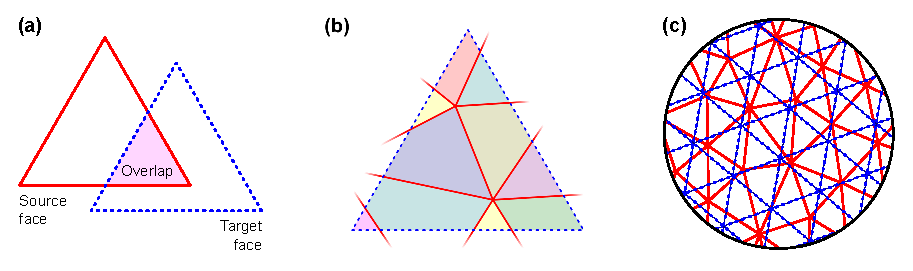
\includegraphics[width=14cm]{images/triangles.eps}
\caption[Overlapping areas used to weight areal quantities during interpolation.]{(\emph{a}) Areal interpolation between a source and a target face uses the overlapping area as a weighting factor. (\emph{b}) For a given target face, each overlapping source face contributes an amount of areal quantity. This amount is determined by the proportion between each overlapping area (represented in different colors) and the area of the respective source face. (\emph{c}) The interpolation is performed at multiple faces of the target surface, so that the amount of areal quantity assigned to a given source face is conservatively redistributed across one or more target faces.}
\label{fig:areal:triangles}
\end{figure}

More specifically, let $Q^{S}_{i}$ represent the areal quantity on the $i$-th face of the registered, source sphere $S$, $i=1,2,\ldots,I$. This areal quantity can be directly mapped back to the native geometry, and can be the area per face as measured in the native geometry, or any other quantity of interest that is areal by nature. Let the actual area of the same face on the source sphere be indicated by $A^{S}_{i}$. The quantities $Q^{S}_{i}$ have to be transfered to a target sphere $T$, the common grid, which face areas are given by $A^{T}_{j}$ for the $j$-th face, $j=1,2,\ldots,J$, $J \neq I$. Each target face $j$ overlaps with $K$ faces of the source sphere, being these overlapping faces indicated by indices $k=1,2,\ldots,K$, and the area of each overlap indicated by $A^{O}_{k}$. The interpolated areal quantity to be assigned to the $j$-th target face is then given by:

\begin{equation}
Q^{T}_{j} = \sum_{k=1}^{K} \frac{A^{O}_{k}}{A^{S}_{k}} Q^{S}_{k}
\end{equation}

Similar interpolation schemes have been devised to solve problems in geographic information systems (\textsc{gis}) \citep{Markoff1973, Goodchild1980, Flowerdew1991, Gregory2010}. Surface models of the brain impose at least one additional challenge, which we address in the implementation (see Section~\ref{sec:areal:implementation}). Differently than in other fields, where interpolation is performed over geographic territories that are small compared to Earth and, therefore, can be projected to a plane with acceptable areal distortion, here we have to interpolate across the whole sphere. Although other conservative interpolation methods exist for this purpose \citep{Jones1999, Lauritzen2008, Ullrich2009}, these methods either use regular latitude-longitude grids, cubed-spheres, or require a special treatment of points located above a certain latitude threshold to avoid singularities at the poles. These disadvantages may render these methods suboptimal for direct use in brain imaging.

\subsection{Implementation}
\label{sec:areal:implementation}

The areal interpolation for spheres is implemented in two parts. In the first, we compute inside of which source faces the target vertices are located, creating a lookup table to be used in the second part. This is the point-in-polygon problem found in vector graphics applications \citep{Vince2005}. Here we calculate the area of each source face, $A^{S}_{i}$, and the subsequent steps proceed iteratively for each face in the source. The barycentric coordinates of each candidate vertex in relation to the current face $i$ is computed; if their sum equals to unity, the point is labelled as inside. However, to test if all vertices are inside every face would needlessly waste computational time. Moreover, since all points are on the surface of a sphere, the vertices in the target are never expected to be coplanar to the source triangular faces, so the test would always fail. The first problem is treated by testing only the vertices located within a bounding box defined, still in the \textsc{3d} space, from the source face extreme coordinates. The second could na\"{i}vely be treated by converting the \textsc{3d} Cartesian coordinates to \textsc{2d} spherical coordinates, which allow a fast flattening of the sphere to the popular plate carr\'{e}e cylindrical projection. However, latitude is ill-defined at the poles in cylindrical projections. Moreover, cylindrical projections introduce a specific type of deformation that is undesired here: straight lines on the surface (geodesic lines) are distorted. The solution we adopt is to rotate the Cartesian coordinate system so that the barycenter of the current source face lies at the point $[r\;0\;0]'$, where $r$ is the radius of the source and target spheres. The barycenter is used for ease of calculation and for being always inside the triangle. After rotation, the current face and the nearby candidate target vertices are projected to a plane using the azimuthal gnomonic projection \citep{Snyder1987}, centered at the barycenter of the face. The point-in-polygon test can then be applied successfully. The key advantage of the gnomonic projection is that all geodesics project as straight lines, rather than loxodromic or other complex paths as with other projections, which would cause many target vertices to be incorrectly labelled. This projection can be obtained trivially after the rotation of the \textsc{3d} Cartesian coordinate system as $\phi=y/x$ and $\theta=z/x$, where $[x\;y\;z]'$ are the \textsc{3d} coordinates of the point being projected. A potential disadvantage of the gnomonic projection is the remarkable areal distortion for regions distant from the center of the projection. Since in typical neuroimaging applications the source and target spheres are composed of a tessellation of approximately $3\times10^6$ faces, $A^{S}_{i} \ll 4 \pi r^2$, and the distortion becomes negligible.

In the second part, the areal interpolation is performed, with the overlapping areas being calculated and used to weigh the areal quantity under study. The identification of intersections between two sets of polygons is also a well studied problem in vector graphics \citep{Guibas1987, Chazelle1994}, which solution depends on optimally finding crossings between multiple line segments \citep{Bentley1979, Chazelle1992, Balaban1995}. Most of the efficient available algorithms assume that the polygons are all coplanar; those that work in the surface of a sphere use coordinates expressed in latitude and longitude and require special treatment of the polar regions. The solution we adopt obviates these problems by first computing the area of each target face, $A^{T}_{j}$; the subsequent steps are performed iteratively for each face in the target sphere, using the azimuthal gnomonic projection, similarly as in the first part, but now centered at the barycenter of the current target face at every iteration. The areal quantities assigned to the faces in the target sphere are initialized as zero before the loop begins. If all three vertices of the current target face $j$ lie inside the same source face $k$, as known from the lookup table produced in the first part, then to the current face the areal quantity given by $Q^{T}_{j} = Q^{S}_{k} A^{T}_{j} / A^{S}_{k}$ is assigned. Otherwise, the source faces that surround the target are examined to find overlaps. This is done by considering the edges of the current target face as vectors organised in counter-clockwise orientation, and testing if the vertices of the candidate faces lie on the left, right or if they coincide with the edge. If all the three vertices of any candidate face are on the right of any edge, there is no overlap and the candidate face is removed from further consideration. If all the three vertices are on the left of all three edges, then the candidate source face is entirely inside the target, which has then its areal quantity incremented as $Q^{T}_{j} \leftarrow Q^{T}_{j} + Q^{S}_{k}$. The remaining faces are those that contain some vertices on the left and some on the right of the edges of the current, target face. The intersections between these source and target edges are computed and false intersections between edge extensions are ignored. A list containing the vertices for each candidate source face that are inside the target face (known for being on the left of the three target edges), the target vertices that are inside each of the source faces (known from the lookup table) and the coordinates of the intersections between face edges, is used to compute the convex hull, using the Quickhull algorithm \citep{Barber1996}. The convex hull delimits the overlapping region between the current target face $j$ and the candidate source face $k$, which area, $A^{O}_{k}$, is used to increment the areal quantity assigned to the target face as $Q^{T}_{j} \leftarrow Q^{T}_{j} + Q^{S}_{k} A^{O}_{k}/A^{S}_{k}$.

The algorithm runs in $\mathcal{O}(n)$ for $n$ faces, as opposed to $\mathcal{O}(n^2)$ that would be obtained by na\"ive search. Nevertheless, the current implementation, that runs in Octave \citep{Eaton2015} or \textsc{matlab} \citep{MATLAB2015}, a dynamically typed, interpreted language, requires about 24 hours to run in a computer with 2.66~GHz Intel Xeon processors.


\subsection{Geodesic spheres and areal inequalities}
\label{sec:areal:geosphere}

The only required feature for the common grid used for the areal interpolation is that all its vertices must lie on the surface of a sphere. The algorithm we present in Section~\ref{sec:areal:implementation} requires further that all faces of the sphere are triangular and that all edges of all faces are much smaller than the radius, so that areal distortion is minimised when projecting to a plane.

A common grid that meet these demands is a sufficiently fine geodesic sphere. There are different ways to construct such a sphere \citep{Kenner1976}. One method is to subdivide each face of a regular polyhedron with triangular faces, such as the icosahedron, into four new triangles. The new vertices are projected to the surface of the (virtual) circumscribed sphere along its radius and the process is repeated recursively a number of times \citep{Lauchner1969}. For the $n$-th iteration, the number of faces is given by $F=4^nF_0$, the number of vertices by $V=4^n(V_0-2)+2$, and the number of edges by $E=4^nE_0$, where $F_0$, $V_0$ and $E_0$ are, respectively, the number of faces, vertices and edges of the polyhedron with triangular faces used for the initial subdivision. For the icosahedron, $F_0=20$, $V_0=12$ and $E_0=30$ (Figure~\ref{fig:areal:geosphere}\emph{a}). For the analyses in this manuscript, we used $n=7$, producing geodesic spheres with 327680 faces and 163842 vertices.

These faces, however, do not have identical edge lengths and areas \citep{Kenner1976}, even though the initial icosahedron was perfectly regular. This is important for areal interpolation, as larger faces on the target grid do overlap with more faces from the source surfaces, absorbing larger amounts of areal quantities, possibly causing confusion if one attempts to color-encode the interpolated image according to the actual areal quantities, in which case, geometric patterns such as in Figure~\ref{fig:areal:geosphere}\emph{b} will become evident. Moreover, smoothing can cause quantities that are arbitrarily large or small due to face sizes to be blurred into the neighbors. Both potential problems can be addressed by multiplying the areal quantity at each face $j$, after interpolation, by a constant given by $4 \pi r^2/(A^{T}_{j}F)$, where $A^{T}_{j}$ is the area of the same face of the geodesic sphere, $F$ is the number of faces, and $r$ is the radius of the sphere.

\begin{figure}[!t]  % Figure 11
\centering
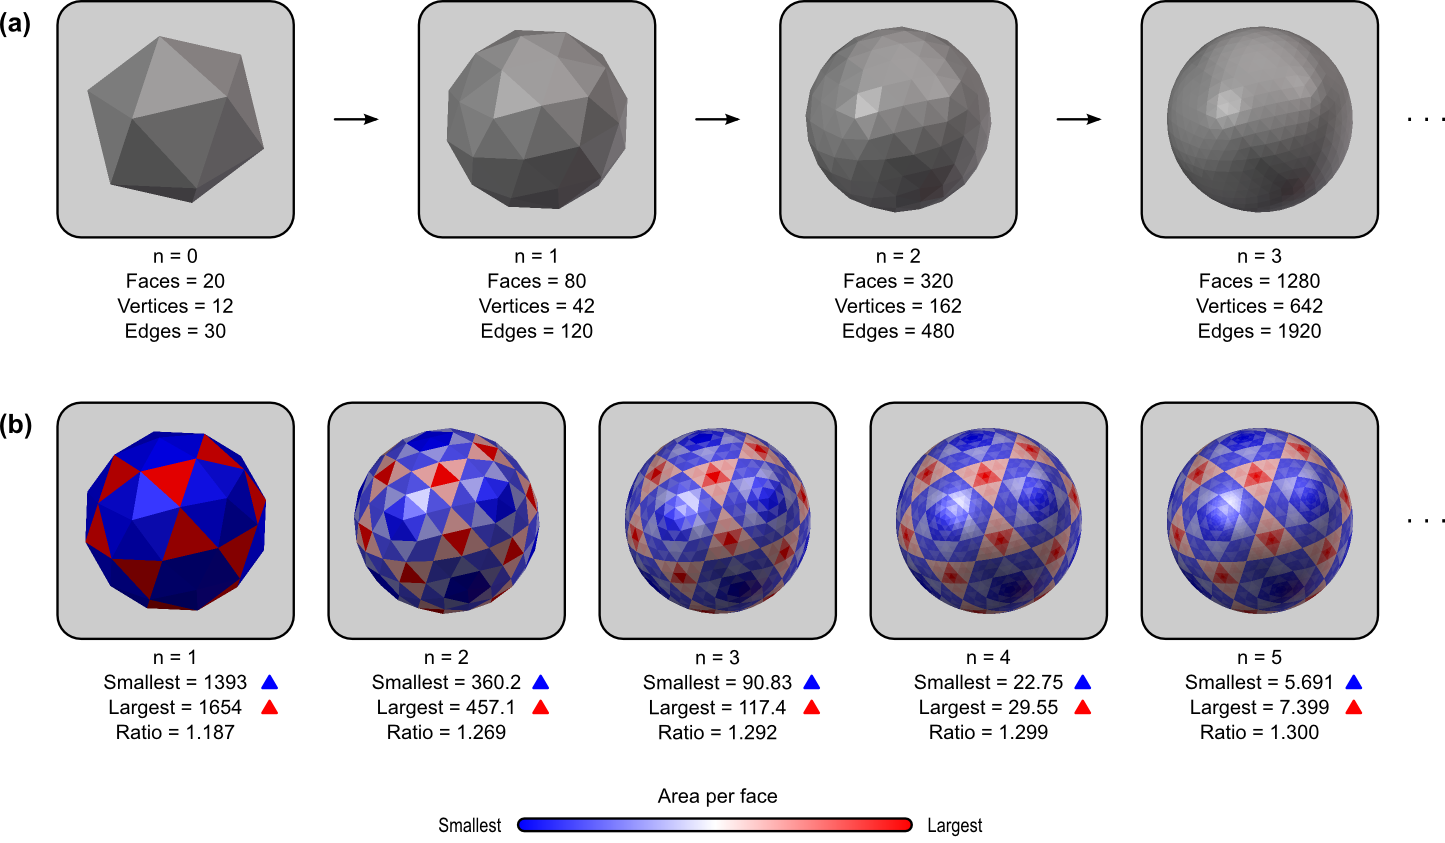
\includegraphics[width=14cm]{images/geosphere.png}
\caption[Geodesic spheres.]{(\emph{a}) The common grid can be a geodesic sphere produced from recursive subdivision of a regular icosahedron. At each iteration, the number of faces is quadruplied. (\emph{b}) After the first iteration, however, the faces no longer have regular sizes, with the largest face being approximately 1.3 times larger than the smallest as $n$ increases.}
\label{fig:areal:geosphere}
\end{figure}

\subsection{Smoothing}
\label{sec:areal:smoothing}

Smoothing can be applied to alleviate residual discontinuities in the interpolated data due to unfavorable geometric configurations between faces of source and target spheres. For the purpose of smoothing, facewise data can be represented either by their barycenters, or converted to vertexwise (see Section~\ref{sec:areal:presentation} for a discussion on how to convert), and should take into account differences on face sizes, as larger faces will tend to absorb more areal quantities (see Section~\ref{sec:areal:geosphere}). Smoothing can be applied using the moving weights method \citep{Lombardi2002}, defined as

\begin{equation}
\tilde{Q}^{T}_n = \frac{\sum_j Q^{T}_j G(g(\mathbf{x}_n,\mathbf{x}_j))}{\sum_j G(g(\mathbf{x}_n,\mathbf{x}_j))}
\end{equation}

\noindent where $\tilde{Q}^{T}_n$ is the smoothed areal quantity at the $n$-th face, $Q^{T}_j$ is the areal quantity assigned to each of the $J$ faces of the same surface before smoothing, $g(\mathbf{x}_n,\mathbf{x}_j)$ is the scalar-valued distance along the surface between the barycenter $\mathbf{x}_n$ of the current face and the barycenter $\mathbf{x}_j$ of another face, and $G(g)$ is the Gaussian kernel.\footnote{As with other neuroimaging applications, smoothing after registration implies that the effective filter width is not spatially constant in native space, neither is the same across subjects. Smoothing on the sphere also contributes to different filter widths across space due to the deformation during spherical transformation.}

\subsection{Conversion from facewise to vertexwise}
\label{sec:areal:conversion}

Whenever it is necessary to perform analyses that include measurements taken at each vertex (such as some areal quantity versus cortical thickness) or when only software that can display vertexwise data is available (Section~\ref{sec:areal:presentation}, it may be necessary to convert the areal quantities from facewise to vertexwise. The conversion can be done by redistributing the quantities at each face to their three constituent vertices. The areal values assigned to the faces that meet at a given vertex are summed, and divided by three, and reassigned to this vertex. Importantly, this procedure has to be done \emph{after} the areal interpolation, since interpolation methods for vertexwise data are not appropriate for areal quantities, and \emph{before} the statistical analysis, since the average of the results of the statistics of a test is not necessarily the same as the statistic for the average of the original data. It should also be observed that conversion from facewise to vertexwise data implies a loss of resolution to approximately half of the original and, therefore, should be performed only if resolution is not a concern and there is no other way to analyse, visualize, or present facewise data or results. The conversion does not change the underlying distribution, provided that the resolution of the initial mesh is sufficiently fine.

\subsection{Statistical analysis}

After resampling to a common grid, the facewise data is ready for statistical analysis. The most straightforward method is to use the general linear model (\textsc{glm}). The \textsc{glm} is based on a number of assumptions, including that the observed values have a linear, additive structure, that the residuals of the model fit have the same variance and are normally distributed. When these assumptions are not met, a non-linear transformation can be applied, as long as the true, biological or physical meaning that underlies the observed data is preserved. In the Evaluation section, we show empirically that facewise cortical surface area is largely not normal. Instead, the distribution is skewed and can be better characterized as \emph{lognormal}. A generic framework that can accommodate arbitrary areal quantities with skewed distributions is using a power transformation, such as the Box--Cox transformation \citep{Box1964}, which addresses possible violations of these specific assumptions, allied with permutation methods for inference \citep[see also Chapter~\ref{sec:perm}]{Holmes1996, Nichols2003} when the observations can be treated as independent, such as in most between-subject analysis.

The application of a statistical test at each face allows the creation of a statistical map and also introduces the multiple testing problem, which can also be addressed using permutation methods. These methods are known to allow exact significance values to be computed, even when distributional assumptions cannot be guaranteed, and also to facilitate strong control over family-wise error rate (\textsc{fwer}) if the distribution of the statistic under the null hypothesis is similar across tests. If not similar, the result is still valid, yet conservative. An alternative is to use a relatively assumption-free approach to address multiple testing, controlling instead the false discovery rate (\textsc{fdr}) \citep{Benjamini1995, Genovese2002}, which offers also weak control over \textsc{fwer}. Other approaches for inference, such as the Random Field Theory (\textsc{rft}) for meshes \citep{Worsley1999, Hagler2006} and the Threshold-Free Cluster Enhancement (\textsc{tfce}) \citep{Smith2009} have potential to be used.

\subsection{Presentation of results}
\label{sec:areal:presentation}

To display results, facewise data can be projected from the common grid to the template geometry, which helps to visually identify anatomical landmarks and name structures. Projecting data from one surface to another is trivial as there is a one-to-one mapping between faces of the grid and the template geometry. The statistics and associated p-values can be encoded in colors, and a color scale can be shown along with the surface model.

However, the presentation of facewise data has conceptual differences in comparison with the presentation vertexwise data. For vertexwise data, each vertex cannot be directly colored, for being dimensionless. Instead, to display data per vertex, typically each face has its color interpolated according to the colors of its three defining vertices, forming a linear gradient that covers the whole face. For facewise data there is no need to perform such interpolation of colors, since the faces can be shown directly on the \textsc{3d} space, each one in the uniform color that represents the underlying data. The difference is shown in Figure~\ref{fig:areal:display}.

\begin{figure}[!tp]  % Figure 12
\centering
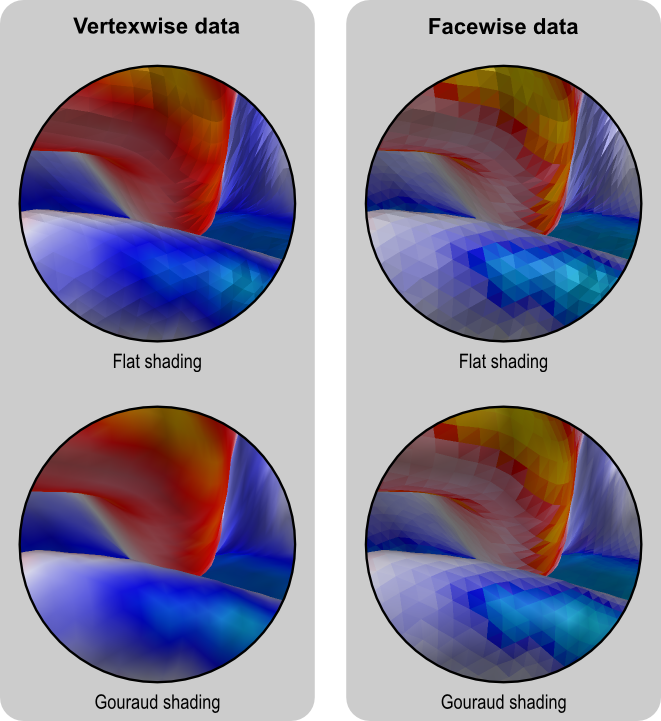
\includegraphics[width=9cm]{images/display.png}
\caption[Differences between presentation of facewise and vertexwise area.]{Differences between presentation of facewise and vertexwise data can be observed in this zoomed portion of the mesh representation of the cortex. Vertices are dimensionless and, to display vertexwise data, the faces have to be colored using linear interpolation. This is not necessary for facewise data, which can be shown directly in the uniform colors that represent the underlying data. In either case, the presentation can be improved by using a shading model, such as Gouraud in this example. Although the vertexwise presentation may be visually more appealing, it contains only half the resolution of the facewise image.}
\label{fig:areal:display}
\end{figure}

Interpolation of colors for vertexwise data should not be confused with the related, yet different concept of lightning and shading using interpolation. Both vertexwise and facewise data can be shaded to produce more realistic images. In Figure~\ref{fig:areal:display} we give an example of simple flat shading and shading based on linear interpolation of the lightning at each vertex \citep{Gouraud1971}.

Currently available software allow the presentation of color-encoded vertexwise data on the surface of meshes. However, only very few software applications can handle a large number of colors per \textsc{3d} object, being one color per face. One example is Blender (Blender Foundation, Amsterdam, The Netherlands), which we used to produce the figures presented in this chapter. Another option, for instance, is to use low-level mesh commands in \textsc{matlab} \citep{MATLAB2015}, such as ``patch''.

\section{Evaluation}

We illustrate the method using data from the Genetics of Brain Structure and Function Study, \textsc{gobs}, a collaborative effort involving the Texas Biomedical Institute, the University of Texas Health Science Center at San Antonio (\textsc{uthscsa}) and the Yale University School of Medicine. The participants are members of 42 families, and total sample size, at the time of the selection for this study, is 868 subjects. We randomly chose 84 subjects (9.2\%), with the sparseness of the selection minimizing the possibility of drawing related individuals. The mean age of these subjects was 45.1 years, standard deviation 13.9, range 18.2--77.5, with 33 males and 51 females. All participants provided written informed consent on forms approved by each Institutional Review Board. The images were acquired using a Siemens \textsc{magnetom} Trio 3~T system (Siemens \textsc{ag}, Erlangen, Germany) for 46 participants, or a Siemens \textsc{magnetom} Trio/\textsc{tim} 3~T system for 38 participants. We used a $T_1$-weighted, \textsc{mprage} sequence with an adiabatic inversion contrast pulse with the following scan parameters: $\textsc{te}/\textsc{ti}/\textsc{tr}$~= 3.04/785/2100~ms, flip angle~= 13$^{\circ}$, voxel size (isotropic)~= 0.8~mm. Each subject was scanned 7 (seven) times, consecutively, using the same protocol, and a single image was obtained by linearly coregistering these images and computing the average, allowing improvement over the signal-to-noise ratio, reduction of motion artifacts \citep{Kochunov2006}, and ensuring the generation of smooth, accurate meshes with no manual intervention. The image analysis followed the steps described in the Methods section, with some variation to test different registration strategies.

\subsection{Registration}

To isolate and evaluate the effect of registration, we computed the area per face after the spherical transformation\footnote{Note that here the area was computed in the sphere with the aim of evaluating the registration method. For analyses of areal quantities, these quantities should be defined in the native geometry, as previously described.} and registered each subject brain hemisphere to a common target using two different registration methods, the Spherical Demons \citep{Yeo2010} and the FreeSurfer registration algorithm \citep{Fischl1999_intersubject}\footnote{The software versions used were \textsc{fs} 5.0.0 and \textsc{sd} 1.5.1.}, each with and without a study-specific template as the target, resulting in four different variants. The study-specific targets for each of these methods were produced using the respective algorithms for registration, using all the 84 subjects from the sample. The non-specific target was derived from an independent set of brain images of 40 subjects, the details of which have been described elsewhere \citep{Desikan2006}. Areal interpolation was used to resample the areal quantities to a common grid, a geodesic sphere produced by seven recursive subdivisions of a regular icosahedron.

The average area per face across subjects was computed after registration and interpolation to identify eventual systematic patterns of distortion caused by warping. This can be understood by observing that, as the vertices are shifted along the surface of the sphere, the faces that they define, and which carry areal quantities, are also shifted and distorted. The registration, therefore, causes displacement of areal quantities across the surface, which may accumulate on certain regions while other become depleted. Ideally, there should be no net accumulation when many subjects are considered and the target is unbiased with respect to the population under study. If pockets of accumulated or depleted areal quantities are present, this means that some regions are showing a tendency to systematically ``receive'' more areal quantities than others, which ``donate'' quantities. The average amount of area after the registration estimates this accumulation and, therefore, can be used as a measure of a specific kind of bias in the registration process, in which some regions consistently attract more vertices, resulting in these regions receiving more quantities. The result for this analysis is shown in Figure~\ref{fig:areal:registration}. Using default settings, \textsc{sd} caused less areal displacement across the surface, with less regional variation when compared to \textsc{fs}. The pattern was also more randomly distributed for \textsc{sd}, without spatial trends matching anatomical features, whereas \textsc{fs} showed a structure more influenced by brain morphology. Using a study specific template further helped to reduce areal shifts and biases. The subsequent analyses we present are based on the \textsc{sd} registration with a study-specific template.

\begin{figure}[!p]  % Figure 4
\centering
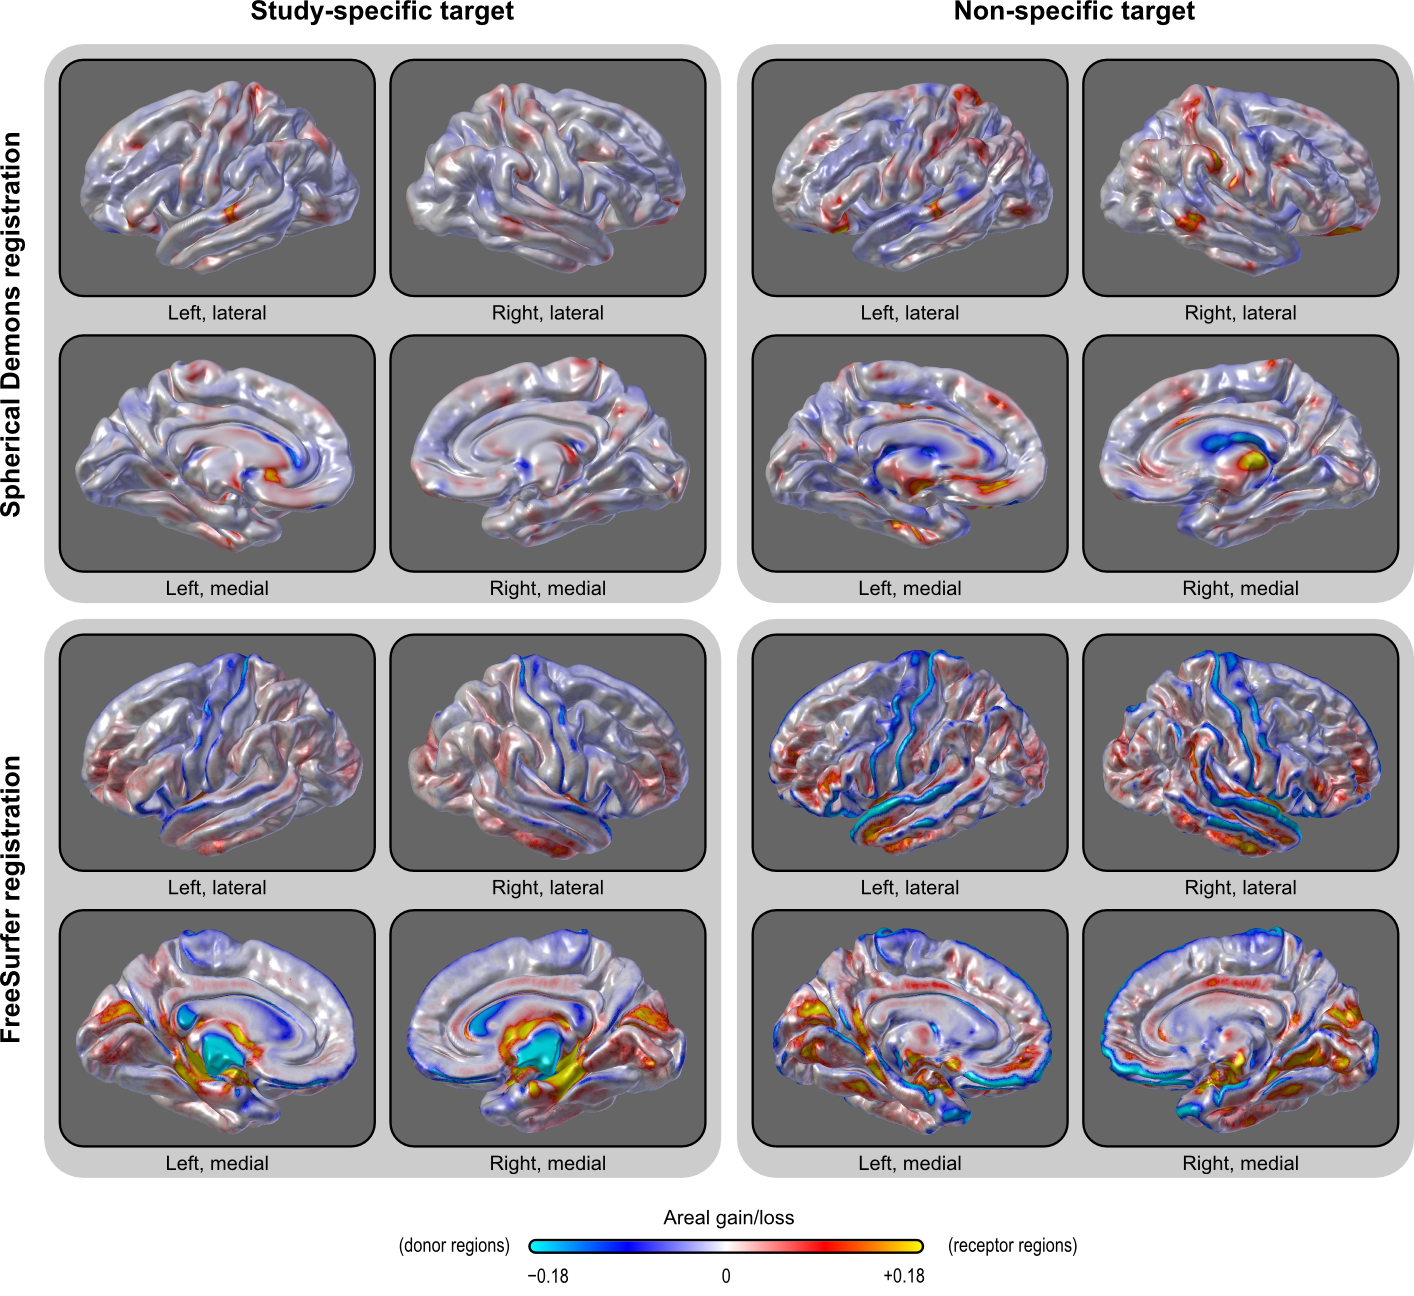
\includegraphics[width=14cm]{images/registration.png}
\caption[Effect of registration method on areal analyses.]{A study-specific template (target for the registration) caused less systematic accumulation of areal quantities across the brain when compared with a non-specific template. Using default parameters, areal accumulation wa less pronounced and unrelated to sulcal patterns using Spherical Demons in comparison with FreeSurfer registration. Gains and losses refer to the area per face that would be expected for areal quantities being redistributed with no bias, i.e. the zero corresponds to the average total surface area of all subjects, divided by the number of faces.}
\label{fig:areal:registration}
\end{figure}

\subsection{Distributional characterization}

To evaluate the normality for the cortical area at the white surface of the native geometry, we used the Shapiro--Wilk normality test \citep{Shapiro1965}, implemented with the approximations for samples larger than 50 as described by \citet{Royston1993}. The test was applied after each hemisphere of the brain was registered to a study-specific template using the Spherical Demons and interpolated to the geodesic sphere using areal interpolation.

For the vast majority of the faces, the area of the white surface is \emph{not} normally distributed (Figures~\ref{fig:areal:shapiro}--\ref{fig:areal:kurtosis-hist}). Instead, the lognormal distribution seems to be more appropriate to describe the data in most parts of the brain, with the test declaring a much larger number of faces as normally distributed after a simple logarithmic transformation. A log-transformation is a particular case of the Box--Cox transformation \citep{Box1964}. For a set of values $y=\left\{ y_1, y_2, \ldots , y_n \right\}$, this transformation uses maximum-likelihood methods to seek a parameter $\lambda$ that produces a transformed set $\tilde{y}=\left\{ \tilde{y}_1, \tilde{y}_2, \ldots , \tilde{y}_n \right\}$ that approximately conforms to a normal distribution. The transformation is a piecewise function given by:

\begin{equation}
\tilde{y} = \left\{ \begin{array}{ll}
\dfrac{y^{\lambda}-1}{\lambda} & (\lambda \neq 0) \\
\ln y & (\lambda = 0)
\end{array} \right.
\end{equation}

Not surprisingly, the Box--Cox transformation rendered the data more normally distributed than a simple log-transformation. However, an interesting aspect of this transformation is that the parameter $\lambda$ is allowed to vary continuously, and it approaches unity when the data is normally distributed, and zero if lognormally distributed, serving, therefore, as a summary metric of how normally or lognormally distributed the data is. Throughout most of the brain, $\lambda$ is close to zero, although with a relatively wide variation (mode = $-0.057$, mean = $-0.099$, sd = $0.493$ for the analysed dataset), indicating that, at the resolution used, the white surface cortical area can be better characterized across the surface as a gradient of skewed distributions, with the lognormal being the most common case. The same was observed for facewise data smoothed in the sphere after interpolation with \textsc{fwhm} = 10~mm (mode = $-0.142$, mean = $-0.080$, sd = $0.578$).\footnote{For scale comparison, the sphere has radius fixed and set as 100~mm, such that the Gaussian filter has an \textsc{hwhm} (half width) = 1.59\% of the geodesic distance between the barycenter of any face and its antipode.} Maps for the parameter $\lambda$ are shown in Figure~\ref{fig:areal:boxcox}.

\begin{figure}[!p]  % Figure Suppl 1
\centering
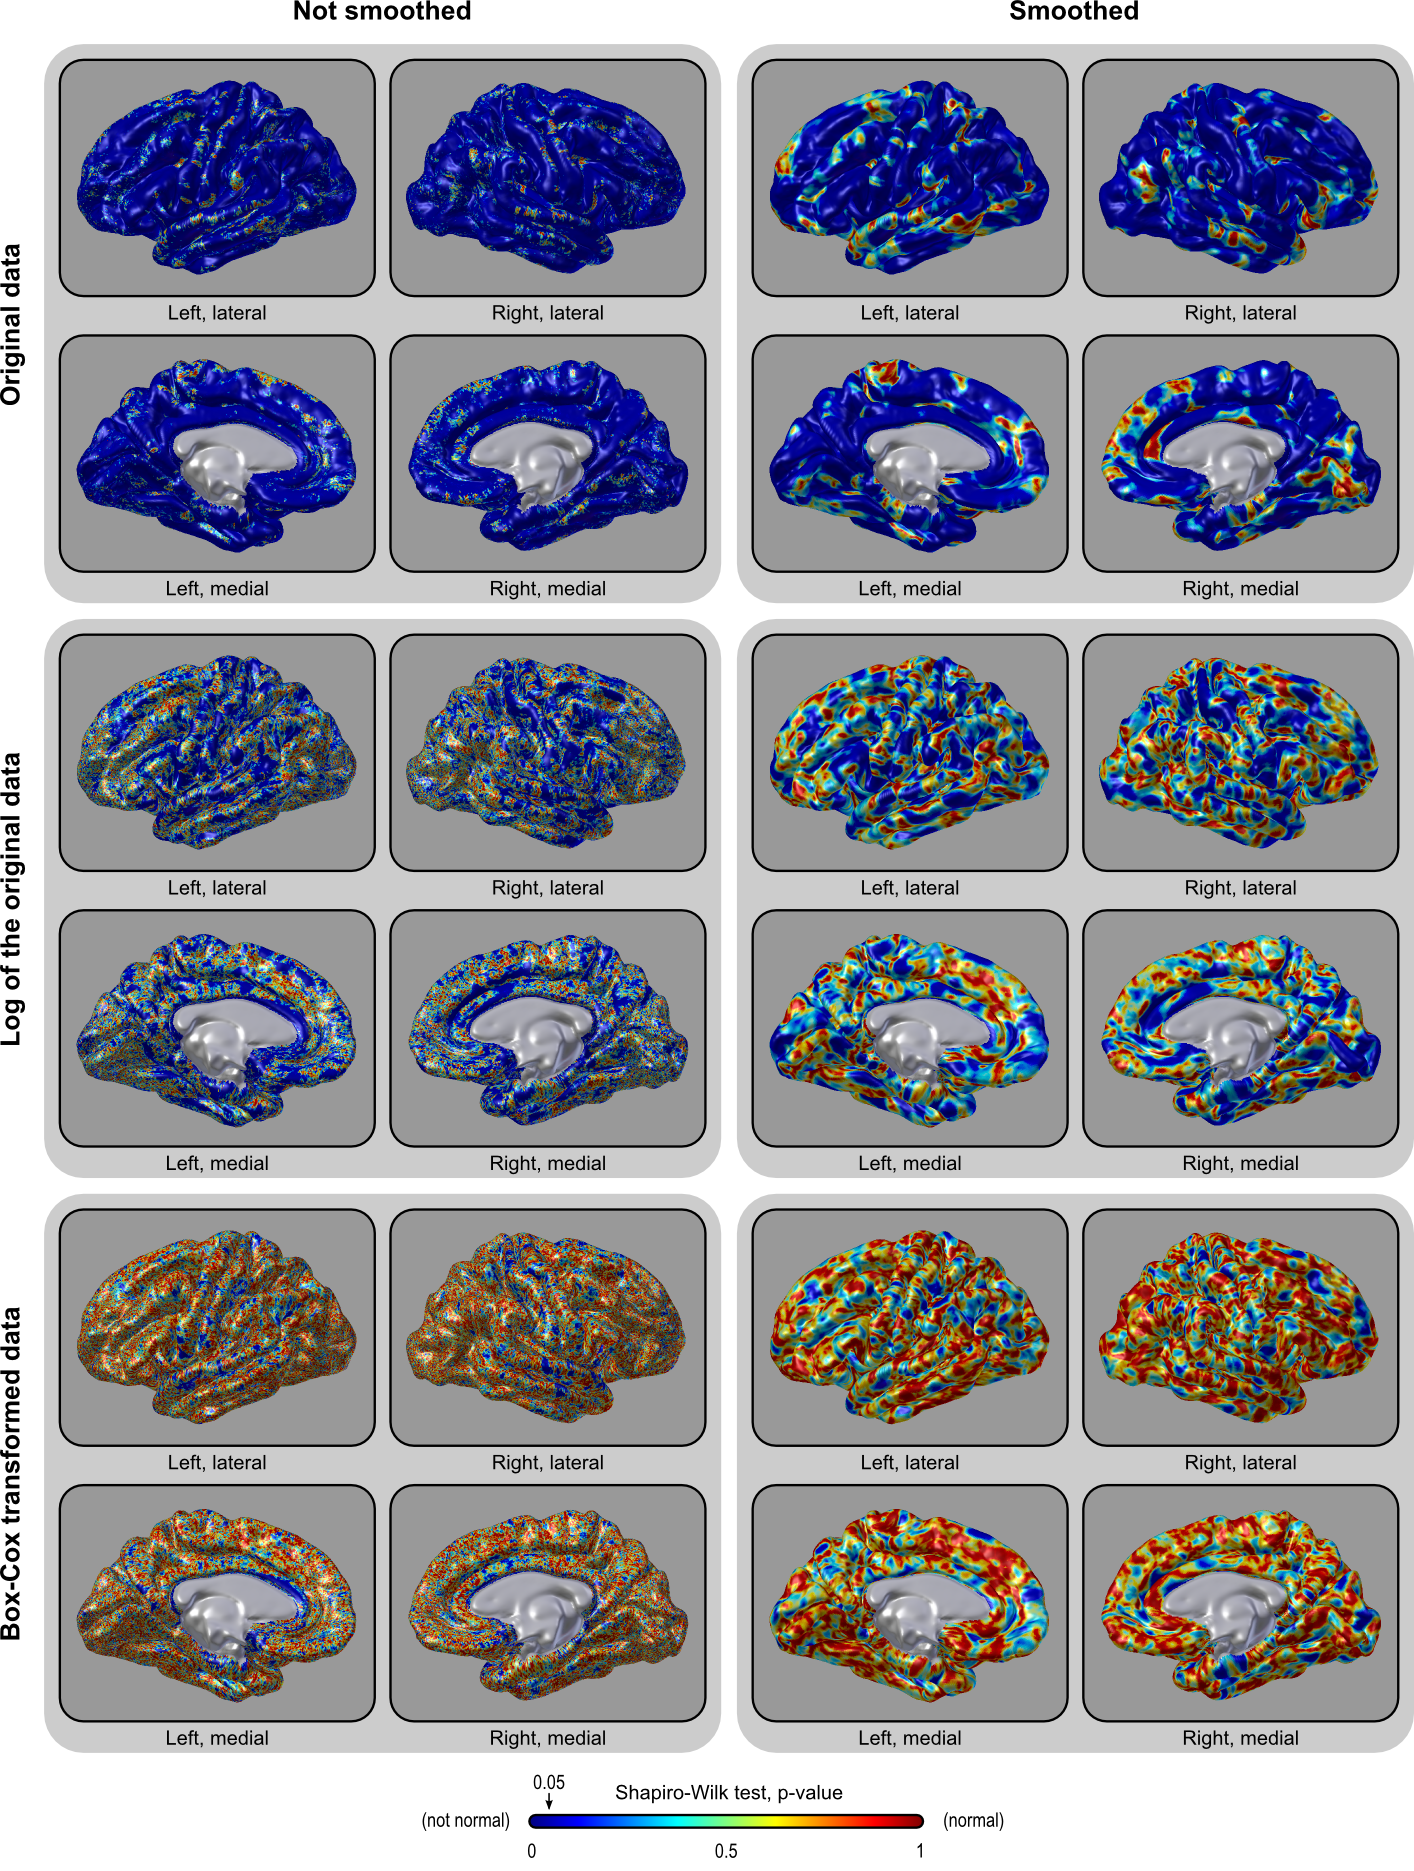
\includegraphics[width=14cm]{images/shapiro.png}
\caption[The distribution of surface area is lognormal.]{The area of the cortical surface is not normally distributed (\emph{upper panels}). Instead, it is lognormally distributed throughout most of the brain (\emph{middle panels}). A Box--Cox transformation can further improve normality (\emph{lower panels}). The same pattern is present without (\emph{left}) or with (\emph{right}) smoothing (\textsc{fwhm} = 10~mm). Although normality is not an assumption for inference as proposed, it offers some advantages, as discussed in the text.}
\label{fig:areal:shapiro}
\end{figure}

\begin{figure}[!p]  % Figure 6
\centering
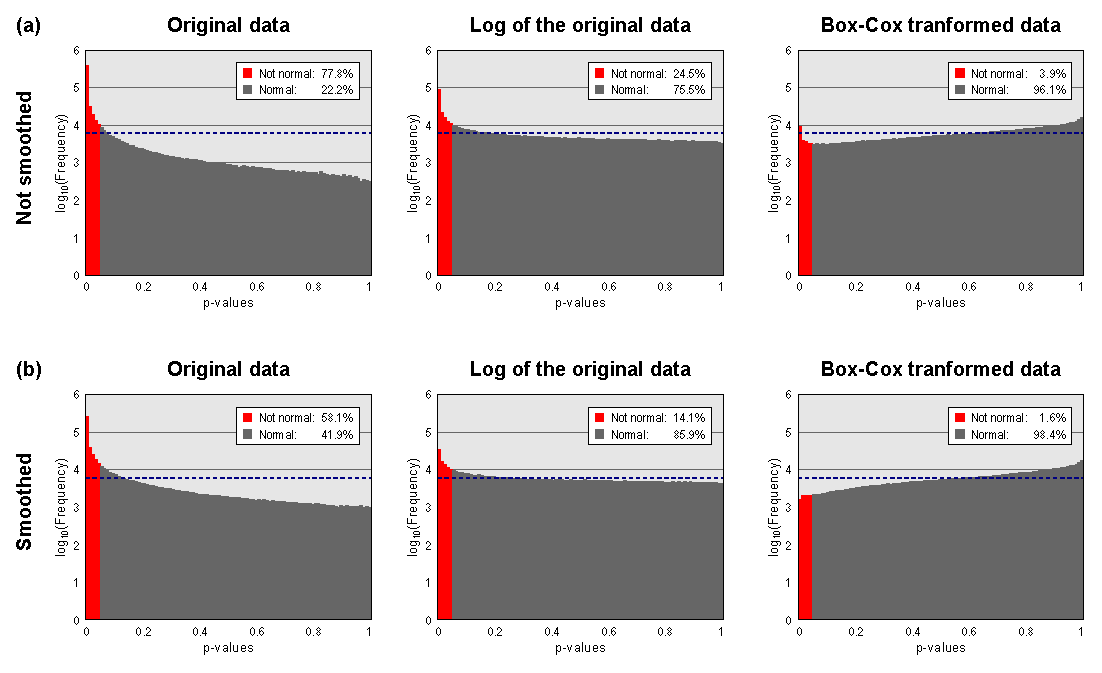
\includegraphics[width=14cm]{images/histograms.eps}
\caption[Results of the Shapiro--Wilk normality test.]{Distribution of the uncorrected p-values of the Shapiro--Wilk normality test. For normally distributed data, 5\% of these tests are always expected to be declared as not normal with a significance level of $\alpha=0.05$. Without transformation or smoothing, near 80\% are found as not normal. Logarithmic and Box--Cox transformations render the data more normally distributed. Observe that the frequencies are shown in logscale. The dashed line (\emph{blue}) is at the frequency that would be observed for uniformly distributed p-values.}
\label{fig:areal:histograms}
\end{figure}

\begin{figure}[!p]  % Figure Suppl 3
\centering
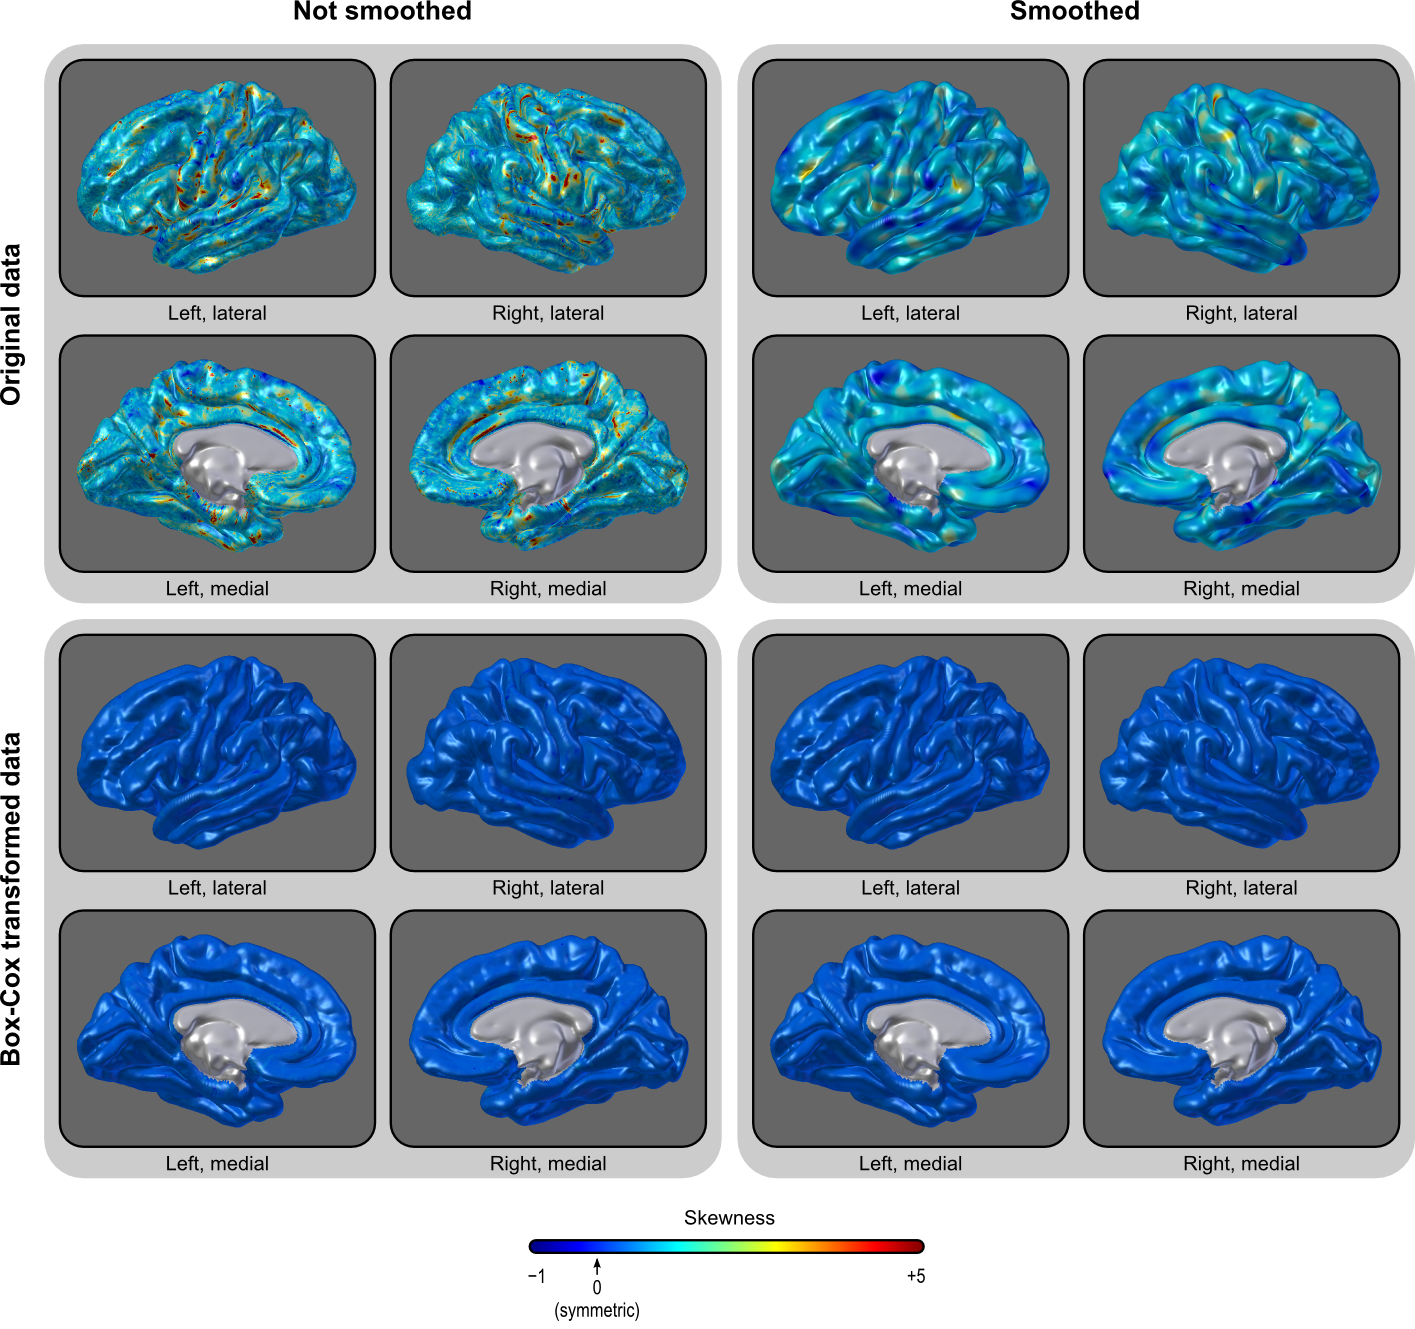
\includegraphics[width=14cm]{images/skewness.png}
\caption[Maps of the skewness of the areal data.]{Maps of the skewness of the areal data, before and after the Box--Cox transformation, and with and without smoothing. The distribution is positively skewed (lognormal) throughout most of the brain, and the transformation successfully brings the data to symmetry (normality). The histograms are shown in Figure \ref{fig:areal:skewness-hist}.}
\label{fig:areal:skewness}
\end{figure}

\begin{figure}[!p]  % Figure Suppl 4
\centering
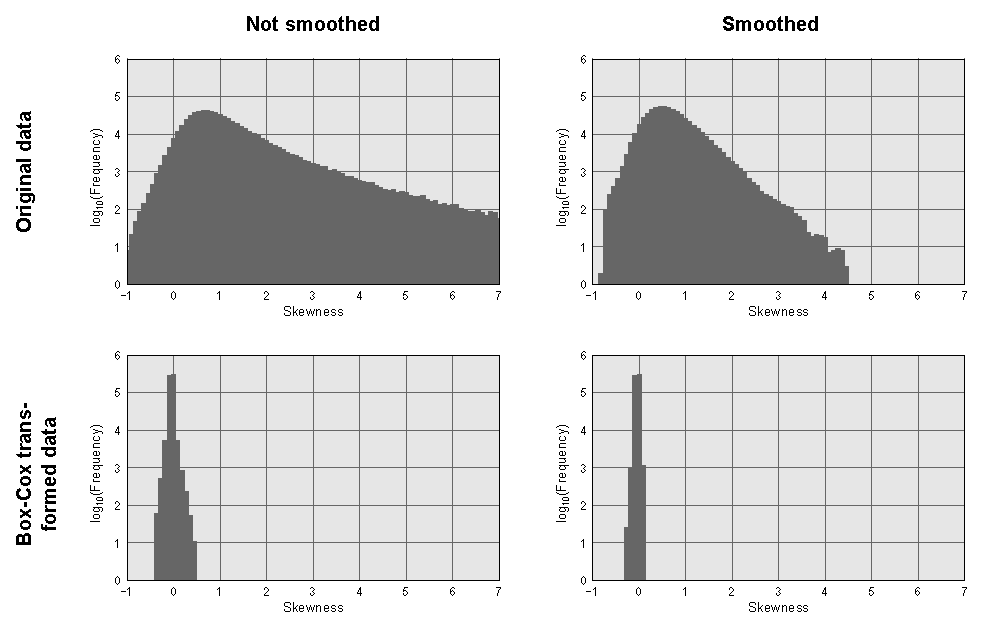
\includegraphics[width=14cm]{images/skewness-hist.eps}
\caption[Histograms of the skewness of the areal data.]{Histograms of the skewness of the areal data, before and after the Box--Cox transformation, and with and without smoothing. The distribution is positively skewed (lognormal) throughout most of the brain, and the transformation successfully brings the data to symmetry (normality). Note that the frequencies are shown in log scale. The corresponding maps are in Figure \ref{fig:areal:skewness}.}
\label{fig:areal:skewness-hist}
\end{figure}

\begin{figure}[!p]  % Figure Suppl 5
\centering
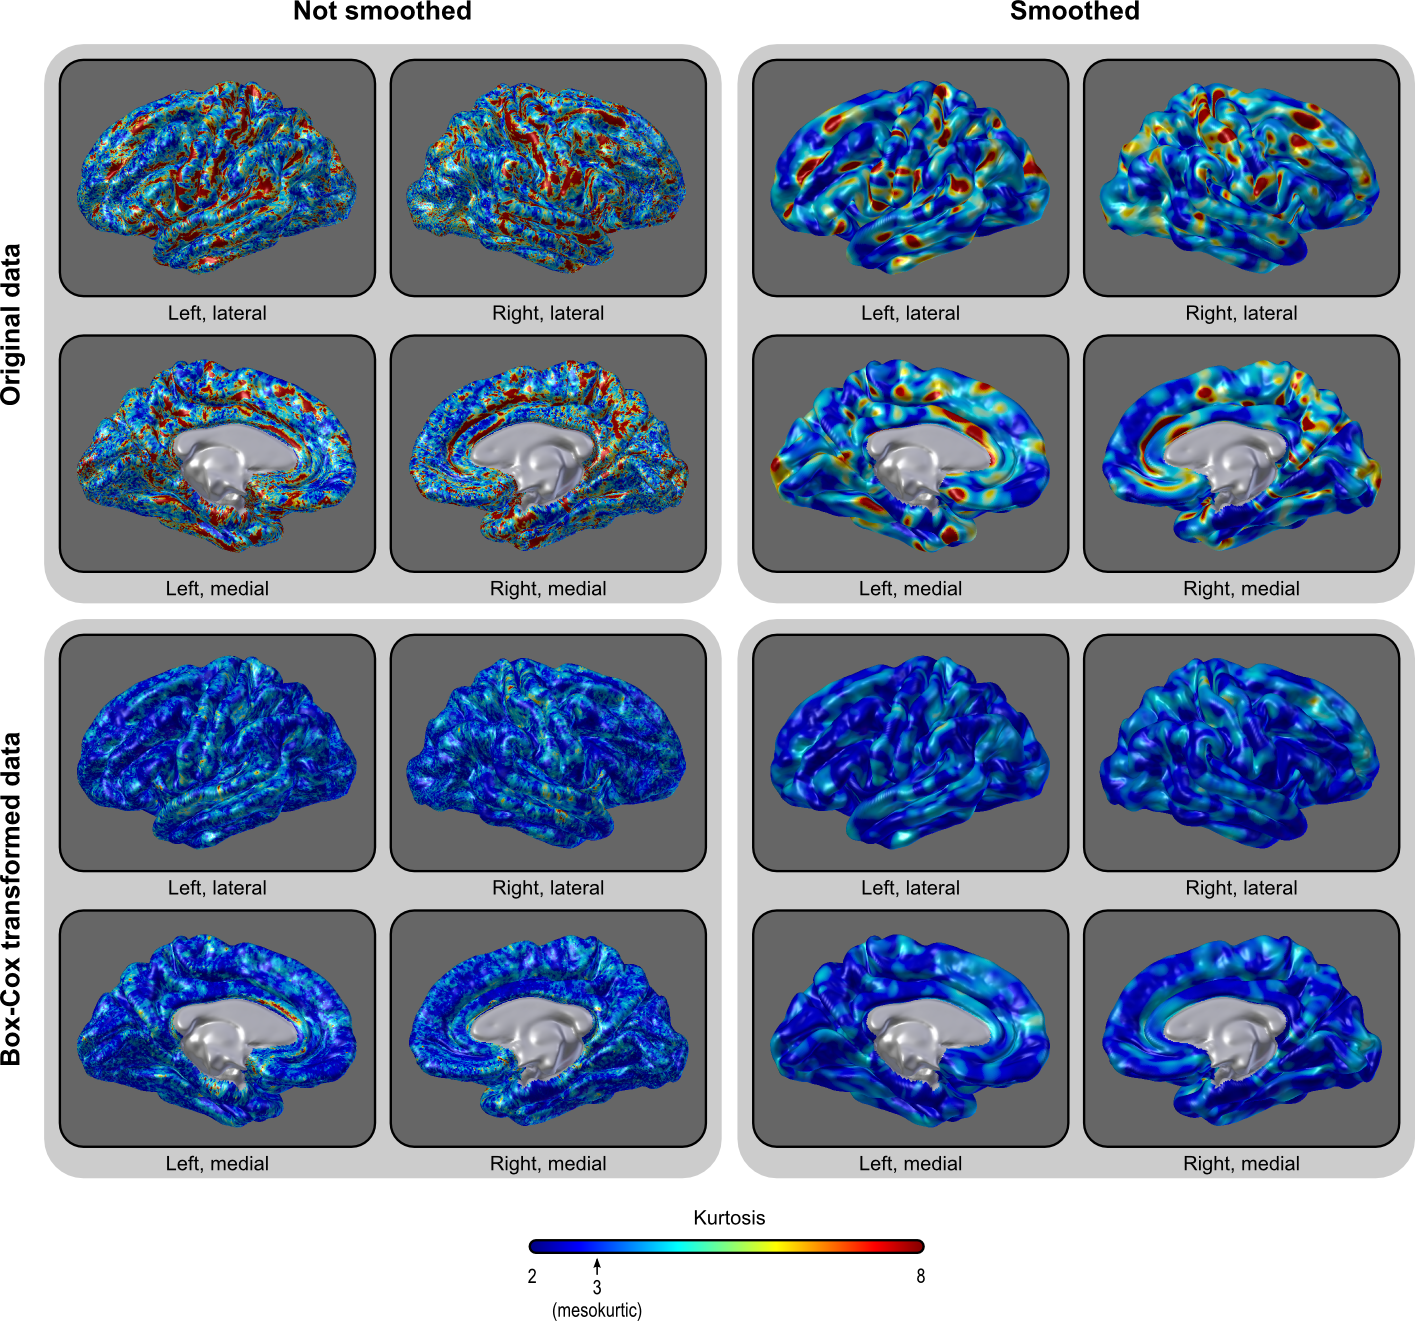
\includegraphics[width=14cm]{images/kurtosis.png}
\caption[Maps of the kurtosis of the areal data.]{Maps of the kurtosis of the areal data, before and after the Box--Cox transformation, and with and without smoothing. The distribution is leptokurtic throughout most of the brain, and the transformation renders the kurtosis closer to the same value as for the normal distribution, i.e.\ closer to the value 3. The histograms are shown in Figure \ref{fig:areal:kurtosis-hist}.}
\label{fig:areal:kurtosis}
\end{figure}

\begin{figure}[!p]  % Figure Suppl 6
\centering
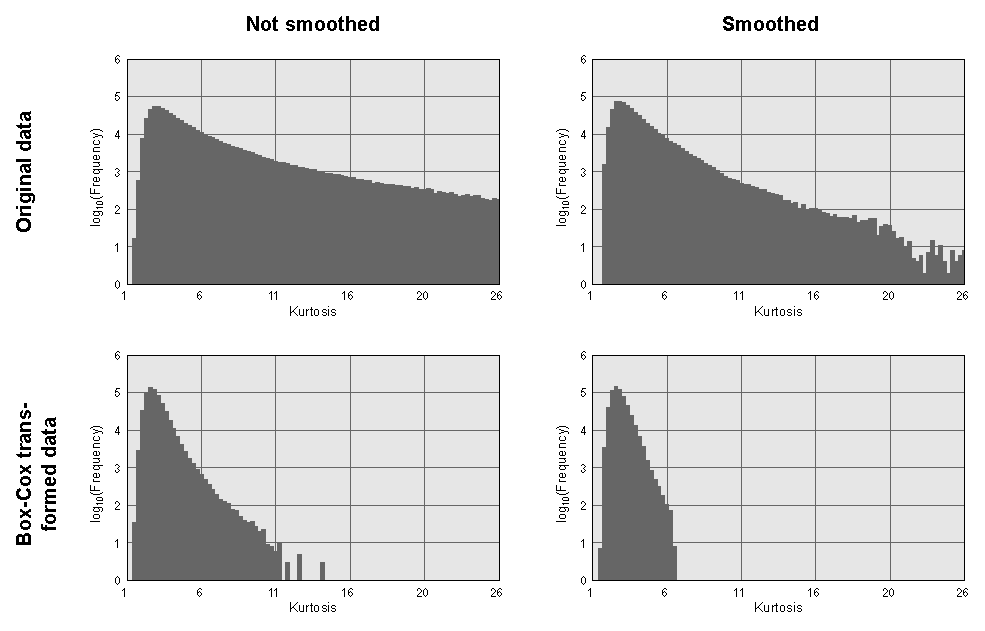
\includegraphics[width=14cm]{images/kurtosis-hist.eps}
\caption[Histograms of the kurtosis of the areal data.]{Histograms of the kurtosis of the areal data, before and after the Box--Cox transformation, and with and without smoothing. The distribution is leptokurtic throughout most of the brain, and the transformation renders the kurtosis closer to the same value as for the normal distribution, i.e.\ closer to the value 3.  Note that the frequencies are shown in log scale. The corresponding maps are in Figure \ref{fig:areal:kurtosis}.}
\label{fig:areal:kurtosis-hist}
\end{figure}

\begin{figure}[!p]  % Figure Suppl 2
\centering
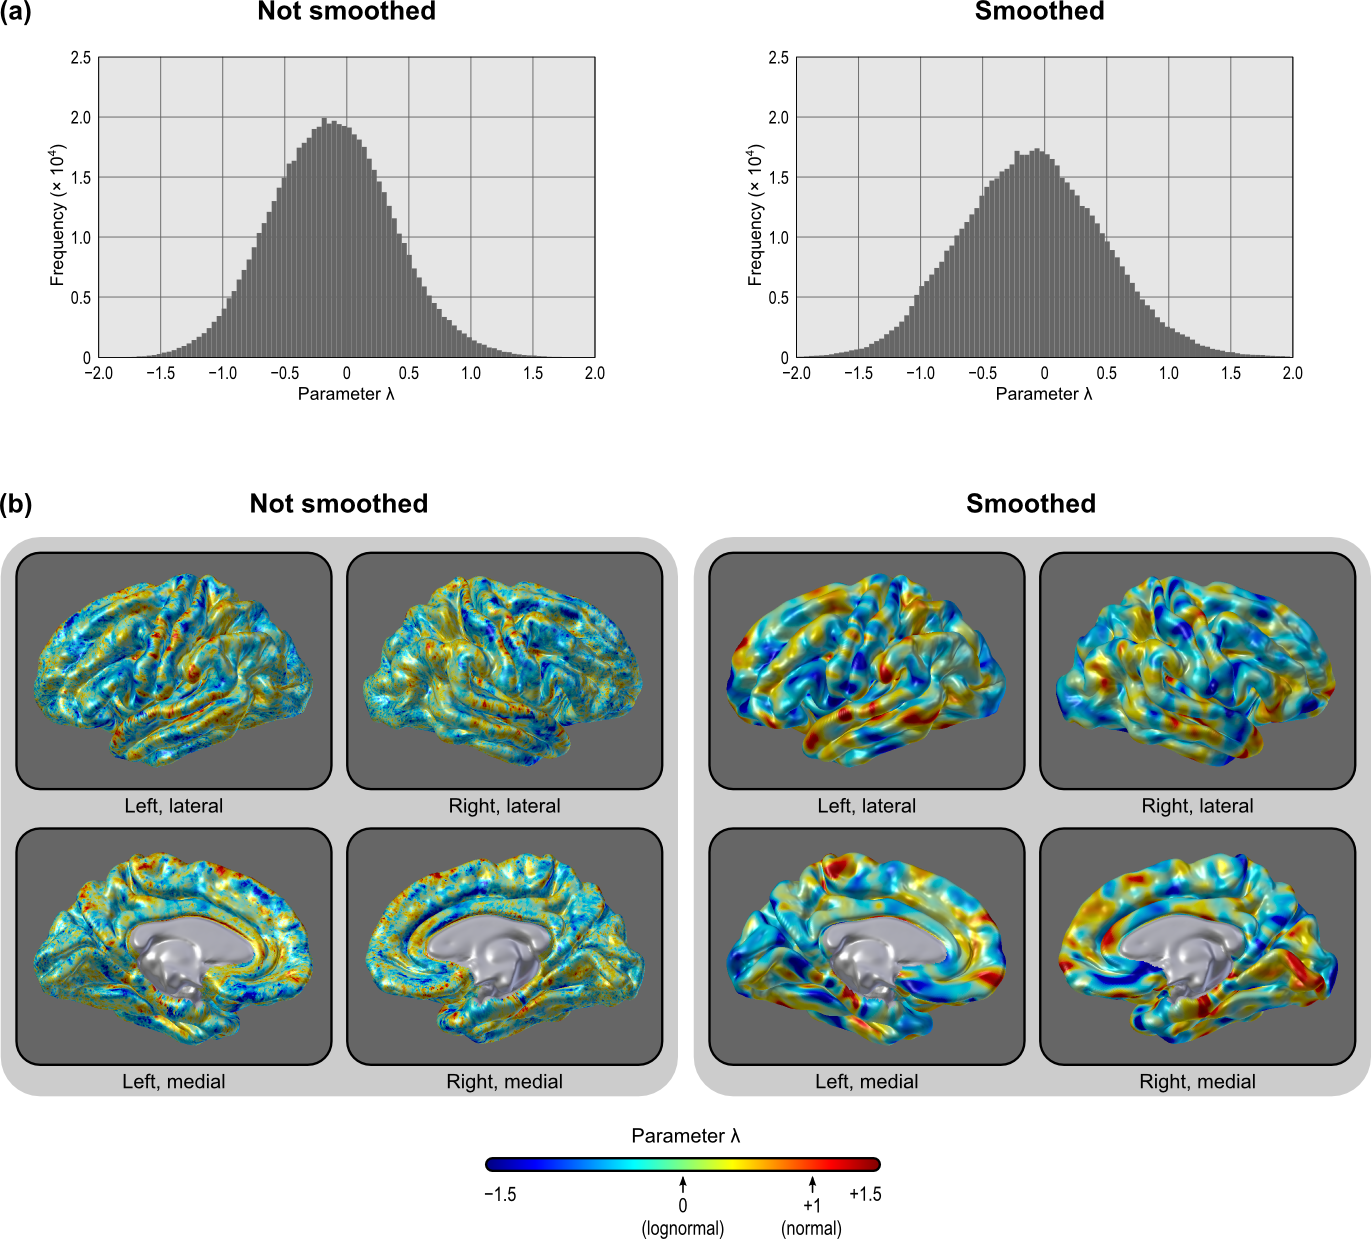
\includegraphics[width=14cm]{images/boxcox.png}
\caption[Spatial distribution of the parameter $\lambda$.]{Distribution of the parameter $\lambda$ of the Box--Cox transformation across the brain: (\emph{a}) histogram and (\emph{b}) spatial map. When $\lambda$ approaches zero, the distribution of the underlying data is more lognormal.}
\label{fig:areal:boxcox}
\end{figure}

\subsection{Comparison with expansion/contraction methods}

A number of studies have analysed what has been called expansion or contraction of the cortical surface when compared to a reference brain. Different studies adopted different operational definitions for what these terms would be [e.g.\ compare \citet{Joyner2009}, \citet{Sun2009}, \citet{Hill2010}], and an unified approach has not been defined. Notwithstanding, the key difference between these methods and the proposed areal analysis is that, at the end of the processing pipeline, areal interpolation ensures the preservation of the amount (mass) of quantities, whereas these methods do not. Moreover, in the framework we present, a number of potential problems that may arise along the pipeline are explicitly addressed. These problems, along with the solutions we propose, are summarized in Table~\ref{tab:areal:compare}.

\begin{table}[!p]
\caption[Problems solved by the proposed method.]{The proposed framework for areal analyses addresses a number of potential problems that may arise along the processing pipeline.}
\begin{center}
{\small
\begin{tabular}{@{}m{42mm}<{\raggedright}m{44mm}<{\raggedright}m{43mm}<{\raggedright}@{}}
\toprule
\textbf{Processing step} &
\textbf{Problem} &
\textbf{Solution} \\
\midrule
Measurements assigned to vertices at the beginning of the analysis. &
Vertices do not hold or convey the same spatial information as the original faces. &
Analyze the faces directly. \\
\midrule
Registration methods that not necessarily produce smooth and invertible warps. &
Discontinuities on expansion or contraction that are not present in the actual brain. &
Use diffeomorphic registration methods. \\
\midrule
Interpolation based on points. &
Areal quantities are not preserved at any scale (local, regional or global). &
Use areal interpolation. \\
\midrule
Use of a standard brain to compute the same measurement that is later analysed. &
Results are interpretable only with respect to that same reference brain. &
Measure and analyse absolute quantities, not relative to some reference. \\
\midrule
Statistical analysis based on assumption of normality. &
The local surface area follows a lognormal distribution. &
Apply a data transformation. Use non-parametric methods. \\
\bottomrule
\end{tabular}}
\end{center}
\label{tab:areal:compare}
\end{table}

With a variety of expansion/contraction methods available, it is difficult to identify the best to which areal analysis could be compared. Here we retessellate the each subject brain in native space using the method described by \citet{Saad2004}. The expansion/contraction method was implemented using the following steps: (1) From the native surface geometry, perform the spherical transformation; (2) Perform the spherical registration to a standard brain; (3) Treat the coordinates $x$, $y$ and $z$ of the vertices from the native geometry as three independent scalar fields over the registed sphere, and interpolate these values to the common spherical grid using barycentric interpolation\footnote{The three scalar fields can also be treated as a single vector field and the barycentric interpolation can be performed in a single step as
\begin{displaymath}
\left[
\begin{array}{c}
x_{P} \\
y_{P} \\
z_{P}
\end{array} \right] = \left[
\begin{array}{ccc}
x_{A} & x_{B} & x_{C} \\
y_{A} & y_{B} & y_{C} \\
z_{A} & z_{B} & z_{C} \\
\end{array}
\right] \left[
\begin{array}{c}
\delta_{A} \\
\delta_{B} \\
\delta_{C}
\end{array} \right]
\end{displaymath} where $x,y,z$ represent the coordinates of the triangular face $ABC$ and of the interpolated point $P$, both in native geometry, and $\delta$ are the barycentric coordinates of $P$ with respect to the same face after the spherical transformation.}; (4) Use the interpolated coordinates, together with the same connectivity scheme between vertices as in the common grid, to construct a new model of the brain in a subject-specific geometry (Figure~\ref{fig:areal:retessellate}); (5) From this new model, compute the area per vertex and divide it by the area per vertex of the homologous point in the template. Call this measurement \emph{expansion/contraction}; (6) Optionally, smooth this quantity.

\begin{figure}[!tbp]  % Figure 7
\centering
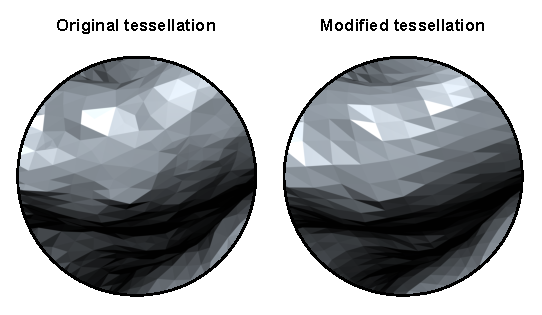
\includegraphics[width=10cm]{images/retessellate.eps}
\caption[Example of a retessellated surface.]{After barycentric interpolation of the coordinates in the surface of the sphere, a new, subject-specific retessellated model is constructed. Areas can be computed directly from the retessellated model and, once divided by the areas of the homologous vertices or faces of the reference brain, constitute the measurement of expansion/contraction.}
\label{fig:areal:retessellate}
\end{figure}

For comparison with the expansion/contraction method, the original facewise area was converted to vertexwise, therefore halving the spatial resolution of the areal data (see Section~\ref{sec:areal:conversion}). In this comparison, we addressed some of the problems presented in Table~\ref{tab:areal:compare}, namely, we registered using Spherical Demons, therefore ensuring smooth and invertible warps, and as target for registration, we used the study-specific template that produced the best results in Figure~\ref{fig:areal:registration}. Furthermore, the measurements were taken at the white surface, rather than the middle surface, as the last is more prone to be influenced by the cortical thickness. It is unclear if, when applicable, these aspects were taken care of in all the different studies that analysed some form of expansion/contraction.

After establishing an expansion/contraction procedure, there are still different ways to compare with areal analysis. The comparison can be made across subjects or across space, can be global or regional, and may or may not include smoothing. In Figure~\ref{fig:areal:expansion} we show that the average amount of area at each vertex did not produce a similar spatial map as the average expansion/contraction. Although the two methods follow remarkably different overall spatial patterns, when vertices across space were pooled together to produce a global measurement, they produced very similar results. Figure~\ref{fig:areal:scatter}a shows the relationship between the global cortical surface area, computed from the sum of the area at each vertex, and a global measure of expansion computed by averaging the expansion/contraction at each vertex across space.\footnote{Note that an exact measurement of expansion/contraction relative to the template can be produced simply by dividing the global area in native geometry by the area of the template geometry. In this case, the points in Figure~\ref{fig:areal:scatter}a would lie in a perfectly straight line, and nothing could be inferred about the relationship between regional variability on expansion estimates and global measurements.} The correlation was very high and helps to validate both methods as a whole. Likewise, when each vertex was analysed separately, the correlation across subjects was also very high, as shown in Figure~\ref{fig:areal:spatialfit}, with an $R^2$ above 0.9 throughout virtually the whole cortex. A spatial comparison of the average maps, on the other hand, showed a very poor relationship between both approaches, as shown in Figure~\ref{fig:areal:scatter}b. When looking at each individual subject, rather than at the average, the correlation across space was still relatively low, albeit not as poor: for the 168 hemispheres analysed, we found an average linear $R^2=0.572$, $\text{sd}=0.044$ without smoothing, and $R^2=0.491$, $\text{sd}=0.065$ after smoothing.

\begin{figure}[!tp]  % Figure 8
\centering
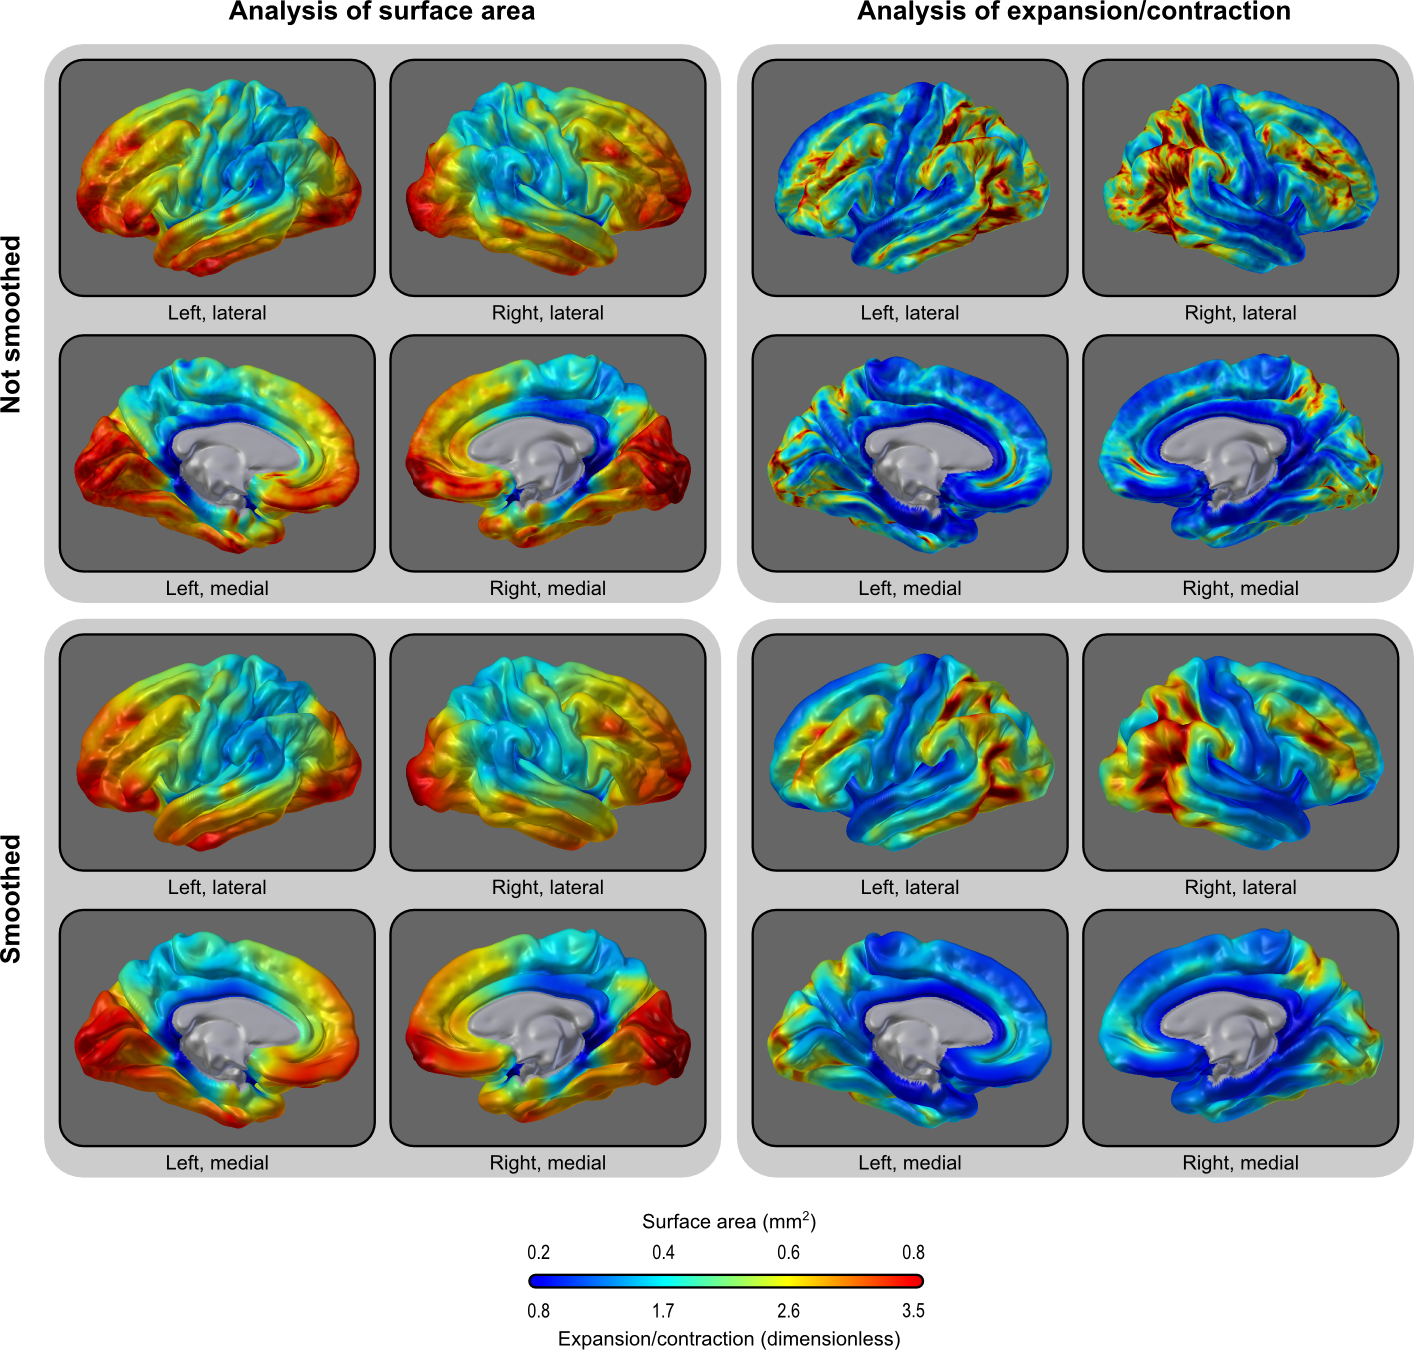
\includegraphics[width=14cm]{images/expansion.png}
\caption[Comparison with expansion/contraction methods (\textsc{i}).]{Average area (\emph{left panels}) or expansion/contraction (\emph{right panels}) per vertex, without (\emph{upper panels}) and with smoothing (\emph{lower panels}). Areal analyses and expansion/contraction differ across space. Smoothing has little global impact.}
\label{fig:areal:expansion}
\end{figure}

\begin{figure}[!tp]  % Figure 9
\centering
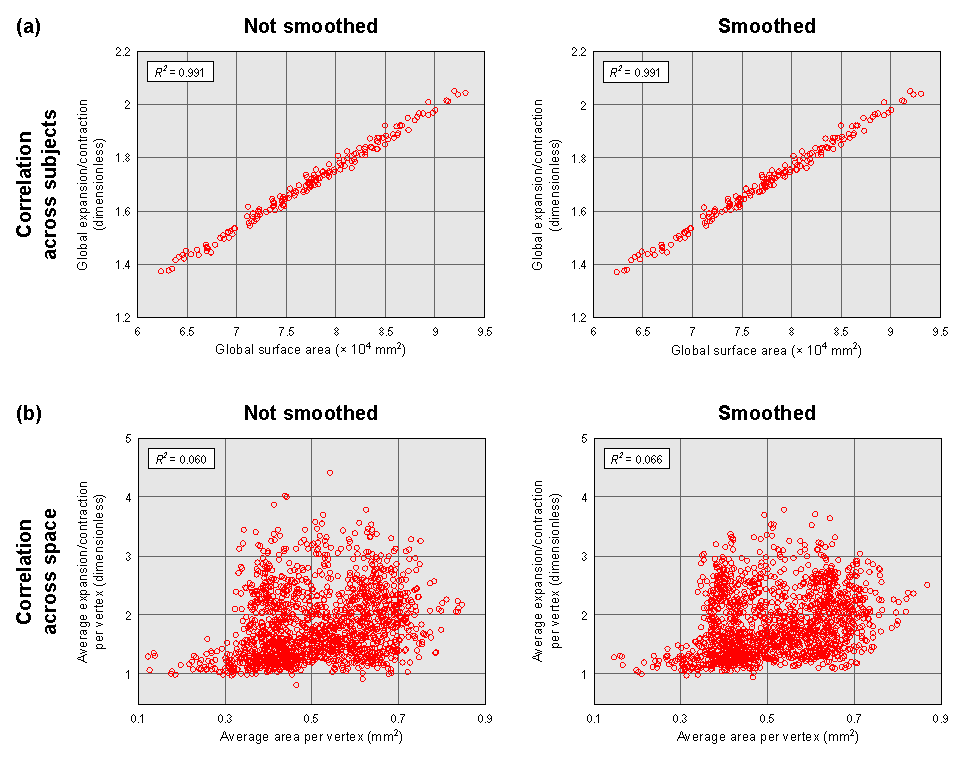
\includegraphics[width=14cm]{images/scatter.eps}
\caption[Comparison with expansion/contraction methods (\textsc{ii}).]{(\emph{a}) The sum of the area per vertex correlates well with the average across space of the expansion/contraction at each vertex (i.e. equivalent to a weighed sum considering each vertex as having the same initial area) for the 168 hemispheres analysed. For the expansion/contraction, this is not the same as computing the ratio between the global surface area in native geometry and of the template, in which case, the result would be a perfectly straight line. The high correlation implies that the regional differences in general compensate each other to produce a similar global effect. (\emph{b}) The correlation between average spatial maps across the 84 subjects, both hemispheres, is very poor between the methods. [Note that, for (\emph{b}), attempts to simultaneously plot all the $>$~300 thousand vertices would not produce meaningful plots in a small space; for this reason only 5\% of the vertices were randomly selected for plotting. The $R^2$ were computed from all vertices and, for both (a) and (b), the value corresponds to the goodness of a linear fit.]}
\label{fig:areal:scatter}
\end{figure}

\begin{figure}[!tp]  % Figure 10
\centering
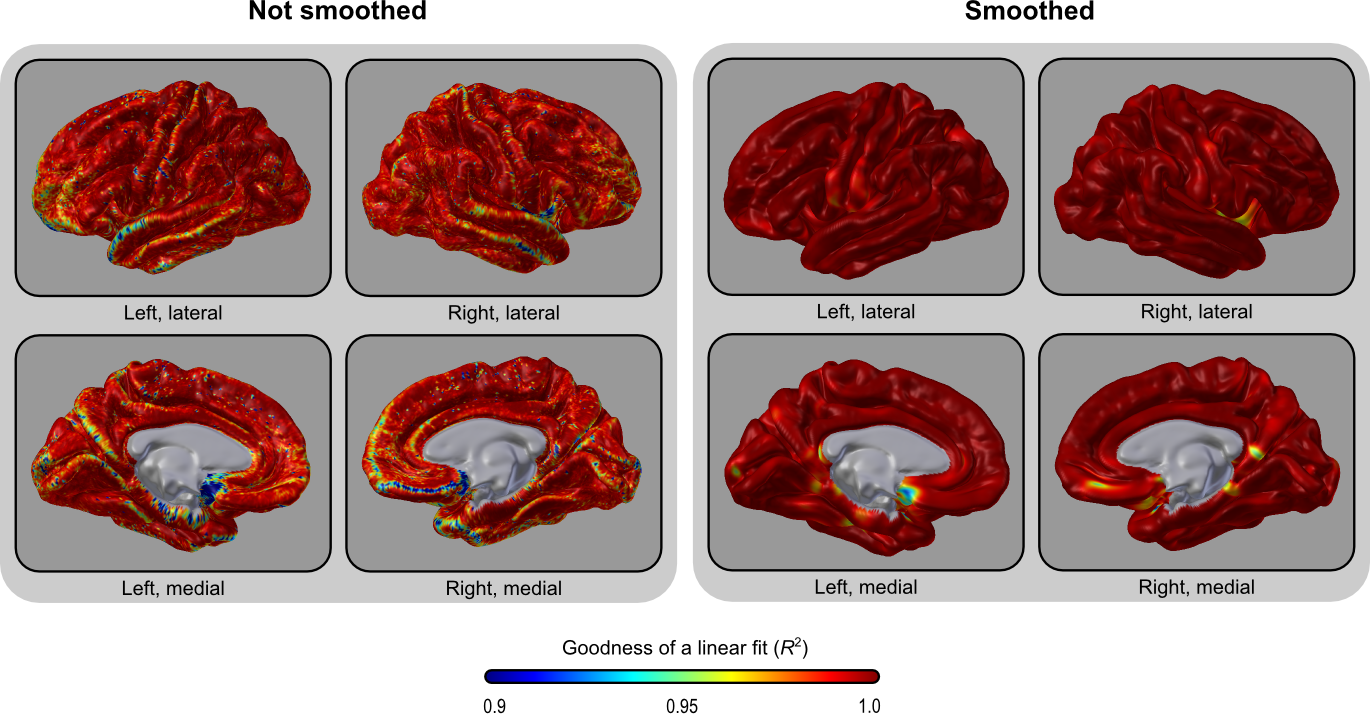
\includegraphics[width=14cm]{images/spatialfit.png}
\caption[Comparison with expansion/contraction methods (\textsc{iii}).]{For each vertex, the linear relationship between areal analyses and expansion/contraction is very high across subjects, being above $R^2=$~0.90 virtually across the whole cortex.}
\label{fig:areal:spatialfit}
\end{figure}

These results suggest that, if each vertex is analysed in isolation, analysis of surface area and analysis of expansion/contraction tend to produce similar results. This is the case, for instance, using mass univariate \textsc{glm}-based approaches. However, for analysis that involve spatial information or that combine information across neighboring vertices, the results are expected to be rather dissimilar. The difference stems from the different units of measurement: areal analyses produce measurements in absolute units of area (e.g.\ mm$^2$), whereas expansion/contraction are relative to the a given reference. The result shown in Figure~\ref{fig:areal:spatialfit}, left panel, also demonstrate, indirectly, that areas measured in the retessellated brain with the resolution used correlate reasonably well with the areas obtained using areal interpolation, and so, have potential to be used as a fast approximation to areal interpolation (Section~\ref{sec:areal:implementation}). Conversely, expansion/contraction measurements can be obtained after areal interpolation simply by dividing the area per face (or per vertex) by its homologous in the reference brain.

\subsection{Validation and stability}

Measurements of surface area are valid as long as the surface reconstruction from \textsc{mr} images produces accurate representations of the cortex. The suggested reconstruction method has been previously validated \citep{Fischl2000}, and is widely used for cortical thickness measurements. Comparison between subjects at the face level depends on good matching of homologies and the registration method we suggest has, likewise, been previously validated \citep{Yeo2010, Klein2010}. As methods evolve, novel approaches for constructing surface representations of the cortex and for registration have potential to improve the overall quality of areal analyses. The validity of areal measurements other than surface area itself depend on each particular measurement technique.

To assess the stability across sessions and scanners, we compared \textsc{mr} images of the same subject acquired in three different sessions collected within a 1 year interval. The imaging protocol varied in terms of acquisition parameters, as well as the number of images used for averaging and improvements on signal and contrast-to-noise ratio. The details are summarized in Table~\ref{tab:areal:retest}. The estimated surface area produced by summing the facewise areas over the cortex after interpolation was very similar across tests, with the largest difference being 8.2\% between Tests \textsc{a} and \textsc{c} (see Table~\ref{tab:areal:retest}), with or without smoothing. The mean and standard deviation for facewise areas were virtually identical across tests, again regardless of smoothing. The pairwise Pearson correlation between the tests for the facewise data after registration and interpolation was above 0.80 without smoothing, and above 0.90 after smoothing with \textsc{fwhm} = 10~mm, showing that the procedure is robust at the face level, even under different scanning conditions and degrees of smoothing.

\begin{table}[!tp]
\caption[Stability of areal measurements.]{Stability and robustness of measurements after registration and interpolation were assessed using three test images of the same subject. The measurements were similar across tests, with similar variability across space and high spatial correlation.}
\begin{center}
{\footnotesize
\begin{tabular}{@{}l@{}m{33mm}<{\centering}@{}m{33mm}<{\centering}@{}m{33mm}<{\centering}@{}}
\toprule
{} & \textbf{Test A} & \textbf{Test B} & \textbf{Test C}\\
\midrule
Manufacturer and model & Siemens~\textsc{magnetom} Trio~3~T & Siemens~\textsc{magnetom} Trio/\textsc{tim}~3~T & Siemens~\textsc{magnetom} Allegra~3~T \\
Sequence & \textsc{mprage} & \textsc{mprage} & \textsc{mprage} \\
\textsc{te/ti/tr} (ms) & 3.04/785/2100 & 2.83/766/2200 & 2.74/900/2500 \\
Flip angle & 13$^{\circ}$ & 13$^{\circ}$ & 8$^{\circ}$ \\
Voxel size (mm) & $0.8 \times 0.8 \times 0.8$ & $0.8 \times 0.8 \times 0.8$ & $1.0 \times 1.0 \times 1.0$ \\
Number of acquisitions & 14 & 7 & 1 \\
Scan date & March 2008 & March 2008 & April 2009 \\
Cortical surface area (mm$^2$) & 176,996 & 177,098 & 180,949 \\
\midrule
\multicolumn{4}{l}{\textbf{Not smoothed}}\\
Average area per face (mm$^2$) & 0.2937 & 0.2939 & 0.3003 \\
Standard deviation             & 0.0938 & 0.0910 & 0.0962 \\
Correlation with Test A        &    --- & 0.8218 & 0.7589 \\
Correlation with Test B        & 0.8218 &    --- & 0.7863 \\
Correlation with Test C        & 0.7589 & 0.7863 &    --- \\
\midrule
\multicolumn{4}{l}{\textbf{Smoothed (\textsc{fwhm} = 10~mm)}}\\
Average area per face (mm$^2$) & 0.2935 & 0.2936 & 0.3000 \\
Standard deviation             & 0.0746 & 0.0712 & 0.0748 \\
Correlation with Test A        &    --- & 0.9509 & 0.9074 \\
Correlation with Test B        & 0.9509 &    --- & 0.9353 \\
Correlation with Test C        & 0.9047 & 0.9353 &    --- \\
\bottomrule
\end{tabular}}
\end{center}
\label{tab:areal:retest}
\end{table}

\section{Discussion}

\subsection{Registration}

To be valid, facewise analyses rely on the assumption that microscopic structures can be localized using as reference the features that are identifiable with \textsc{mri} and which drive the registration. Features with such localizing power are important because they help to ensure good overlap of homologous areas between subjects. Despite an implicit assumption already present in most imaging studies, only recently it has been demonstrated valid for some cytoarchitetonic areas when the references are the cortical folding patterns, even though for non-primary regions, the mismatch may still be substantial \citep{Fischl2008, Fischl2009, Hinds2008, Hinds2009, DaCosta2011}. Other features, some microscopic and detectable only under ultra-high field strengths \citep{Augustinack2005, Bridge2006, Duyn2007, Kim2009}, have the potential to be used as the reference as long as they are demonstrated to be markers of histologically or functionally defined areas, possibly replacing folding patterns altogether, or used to provide ancillary information. Myeloarchitectural features may be particularly useful for this application, for being resposible for most of the contrast observed with \textsc{mri} \citep{Geyer2011}. Likewise, areal analyses can be conducted after registration based on features derived from functional \textsc{mri} \citep{Sabuncu2010}.

Good matching of homologies, however, depends not only on the features used to guide the registration, but on the registration method itself. For facewise areal analyses, invertibility is necessary to prevent faces from being folded over others. In addition, methods that produce smooth warps are necessary to ensure that areal quantities are transferred smoothly, without abrupt variations. Such abrupt variations would only be acceptable if matching perfectly with areas where structure and/or function also changes abruptly. A spatial transformation that allows such perfect matching, however, cannot be obtained easily in practice, since these borders usually cannot be observed with current, conventional \textsc{mri} methods, and importantly, since many of the differences between regions are subtle and the transitions are gradual. However, invertibility and smoothness, as guaranteed by diffeomorphic methods, albeit important, may not suffice. Our results show that even methods that produce smooth varying warps can differ substantially with respect to how the areal quantities are shifted across the surface. It is possible that performance differences between these methods might be due to choices on regularization strategies and associated parameters \citep{Fischl1999_intersubject, Yeo2010}, instigating further reseach on selections that may produce the most accurate results \citep{Yeo2010b}. Our experiments also demonstrate that the choice of the target used for registration affects the distortion in areal measurements.

\subsection{Areal interpolation}

Areal interpolation allows direct analysis of areal quantities in absolute values, including the surface area itself. This is because it is the areal quantity proper that is conservatively transfered between grids. Therefore, there is no need to apply corrections due to stretches or shrinkages, such as using the Jacobian of the transformation \citep{Good2001}, nor due to the choice of the parametrizable surface \citep{Thompson1999}. Moreover, the results are interpretable directly with regard to the actual amount of tissue or other measurement under study, rather than relative to concepts as expansion/contraction, which are always relative to a given reference, and can create difficulties in interpretation and comparison across studies, either due to different definitions adopted by different authors, or due to the the need of a reference brain. Notwithstanding, after areal interpolation, it continues to be possible to divide the areas by the areas of the homologous faces or vertices of a reference brain, and so, obtain an expansion/contraction measurement. Moreover, areal quantities that are not area itself can also be divided by the area of each face or vertex in native geometry, thus converting these quantities to densities if necessary.

It should be emphasized that, as with other interpolation strategies, areal interpolation is not perfectly reversible, i.e.\ once the cortical area of a subject is transferred to a different grid, remapping back to the subject surface will not produce locally identical results, although the global areal quantity is always conserved. This is because within each face, the areal quantity is implicitly assumed to be homogeneously distributed. This only becomes a problem if low resolution meshes are used and if several back-and-forth iterations are performed.

\subsection{Statistical analysis of areal quantities}

There are a number of reasons that go beyond purely methodological considerations to justify the transformation of the data before statistical analysis. Measurements related to biological morphology, such as lengths, areas, volumes or weights, are well known to follow non-normal distributions. If the diameter of a structure, for instance, is normally distributed, inevitably both its cross section and its surface area follow skewed distributions, whereas its volume follows an even more skewed \citep{Kapteyn1916, Gaddum1945}. All these related measurements cannot be normally distributed simultaneously. The skewness is higher when the variability is relatively large in comparison to the measure of central tendency that best describes the data, such as the arithmetic or the geometric mean. If the non-normality is not considered, statistical models are likely to produce inaccurate results. In this scenario, a power transformation, such as the Box--Cox transformation, helps to identify subjacent, possibly causative, normally distributed effects.

The lognormal distribution, more specifically, is known to arise in a variety of biological processes. Of particular interest is the autocatalytic growth of tissue over time. The number of cells present on a tissue that grows in an unrestricted way can be given by the familiar formula $N=N_0e^{ct}$, where $N_0$ is the initial number of cells, and $t$ is the amount of time in which the cell grows under the circumstances represented by the constant $c$, a factor that incorporates a variety of influences, such as genetic and environmental. $N$ will be lognormally distributed if either $c$ or $t$ are normally distributed \citep{Koch1966, Limpert2001}. The finding that the facewise cortical surface area follows mostly lognormal distributions may suggest that the method may capture these biological effects. Such interpretation can only subsist under the tenets of accurate and smooth registration.

From a statistical perspective, permutation methods do not rely on normality, rendering them appropriate in a variety of situations in which this assumption is not tenable. Nevertheless, the data should, still, undergo a transformation. As discussed above, the reason is not merely to conform to normality, although that comes as a bonus, but also to ensure that underlying biological effects, either multiplicative or proportionally dependent upon an initial value, can be treated as additive in a linear model \citep{Christensen2002}. Areal quantities that are not the cortical surface area itself can, notwithstanding, be distributed differently, and the framework for statistical analysis outlined in the Methods section appears generic enough to accomodate a variety cases. The Box--Cox transformation has yet another advantage when used in combination with permutation methods under multiple testing conditions: the more stable variance after the transformation allows the distribution of the statistic under null hypothesis to become more similar across tests, allowing \textsc{fwer} to be controlled at a level closer to its nominal value using the distribution of the maximum statistic.

\subsection{Box--Cox and log-normality}

An interesting aspect related to the Box--Cox transformation is that here it was used as a metric to quantify how normal or log-normal the data are. This has clear applications in biology. Tissue growth that depends on cellular multiplication is exponential, with a constant factor that is often normally distributed, resulting in tissue size that is log-normally distributed \citep[for a discussion, see][]{McAlister1879, Koch1966, Koch1969}. Measurements of the final tissue size in different individuals, however, does not perfectly conform to the log-normal due to external influences that may hinder tissue growth. Moreover, it is not always possible to measure the final amount of tissue that is the product of a single lineage of self-multiplicative cells. The combination of different cell lineages, each with their own growth rate, as well as external influences, tend to produce a distribution that is more normally (Gaussian) distributed. This appears to be the case of the cerebral cortex, with a \emph{distribution gradient} between these two extremes of normality and log-normality. Estimating the parameter $\lambda$ allows one to estimate also how closer to normal or log-normal certain measurements are. If $\lambda \approx 0$, the original data tend to be log-normally distributed, whereas if $\lambda \approx +1$, the data can be considered approximately more normally distributed.

\subsection{Further developments and potential applications}

Facewise analyses offer the possibility of studying surface area at a much finer scale than previously. This is a feature of interest in many research fields across the neurosciences, as well as in medicine. Although the same applies to vertexwise cortical thickness, thickness and area provide different and complementary insights into processes underlying the development of the brain and disorders \citep{Voets2008, Winkler2010, SanabriaDiaz2010}.

Provided that the neurons in the cortex retain largely their same relative positions as the progenitor cells in the embryo \citep{Rakic1988, Rakic2009a, Pierani2009, Clowry2010}, facewise comparison of surface area allows one to hypothesize about ontogenetic processes to the extent that they can be observed and localized with \textsc{mri}, even long after the end of phases of massive tangential cellular proliferation. Until now, this kind of study could not be performed, either due to lack of methods to analyse cortical surface area without the constrains imposed by regions of interest, or due to inherent limitations of methods based on expansion or contraction.

The study of local cortical surface area offers, moreover, new possibilities for connectivity analyses, as the need for parcellations based on macroscopic anatomy is obviated. Indeed, the results of connectivity analyses are known to be influenced by the choice of the parcellation that define nodes of putative neuronal networks \citep{Butts2009, Rubinov2010}. Notwithstanding, if a given set of regions is derived from a different method \citep{Beckmann2009a, Nelson2010}, these can be directly associated with their corresponding surface-based areas or areal quantities by means of areal interpolation.

Another potential application is for genetic analyses. Given that cortical surface area and thickness are both heritable, yet genetically not correlated \citep{Panizzon2009, Winkler2010}, these traits, separately, can be used in a framework similar to voxelwise genome-wide association studies (v\textsc{gwas}) \citep{Stein2010}. Identification of genes that influence surface area have potential to elucidate a myriad of developmental, neurologic and psychiatric disorders.

\section{Chapter conclusion}

We presented an interpolation method for between-subject analyses of cortical surface area. The method is also suitable for other quantities that are areal by nature and which require mass conservation (pycnophylactic property) during interpolation and analysis. We demonstrated that, when the quantity under study is surface area itself, the distribution of the data does not follow a normal distribution, being instead better characterized as lognormal, and proposed a framework for statistical analysis and inference.